\documentclass[11pt,a4paper]{article}

% ---------- arxiv-style preamble (xelatex; emoji-native) ----------
\usepackage[margin=1in]{geometry}
\usepackage{amsmath,amssymb,amsthm}
\usepackage{graphicx}
\usepackage{booktabs}
\usepackage{longtable}
\usepackage{siunitx}
\usepackage{hyperref}
\usepackage{xcolor}
\usepackage[numbers,sort&compress]{natbib}
\usepackage{tikz}
\usetikzlibrary{positioning,arrows.meta,fit,backgrounds}
\usepackage{caption}
\captionsetup{font=small,labelfont=bf}
\usepackage{listings}
\usepackage{array}
\lstset{
  basicstyle=\ttfamily\footnotesize,
  breaklines=true,
  columns=fullflexible,
  frame=single,
  framesep=4pt,
  xleftmargin=4pt,
  xrightmargin=4pt
}
\hypersetup{
  colorlinks=true,
  linkcolor=blue!50!black,
  citecolor=blue!50!black,
  urlcolor=blue!50!black
}

% ---------- tier badges (xelatex; colored-disc fallback) ----------
% Use \tierBlue / \tierGreen / \tierYellow / \tierOrange / \tierRed in tables.
% Rendered as filled colored discs via TikZ (engine-agnostic, always visible,
% preserves the exact tier semantics: blue=closed-form, green=numerical, etc.).
\newcommand{\tierdisc}[1]{\textcolor{#1}{\rule[0.05ex]{1.0ex}{1.0ex}}}
\newcommand{\tierBlue}{\tierdisc{blue!70!black}}
\newcommand{\tierGreen}{\tierdisc{green!60!black}}
\newcommand{\tierYellow}{\tierdisc{yellow!85!black}}
\newcommand{\tierOrange}{\tierdisc{orange!90!black}}
\newcommand{\tierRed}{\tierdisc{red!80!black}}

\title{
  \textbf{ANTIMATTER FACTORY: A 7-Process Closed-Form Verify Funnel
  for Cold-Antihydrogen Production and a CPT-Test Design Feasibility} \\[6pt]
  \large with a Penning-Trap Three-Frequency Invariance Keystone, an Inherited
  RTSC Magnet Toolchain at the Confinement Stage, and an Algebraic-Root
  \textsc{Blue-Max} Audit
}

% ---------- author block (hexa-codex style) ----------
% Convention: <repo> maintainers / dancinlab / clickable github URL.
% LLM collaborator credit goes in \paragraph{Acknowledgments} at the tail.
\author{
  \texttt{antimatter-factory} maintainers\\
  \normalsize\textit{dancinlab}\\[2pt]
  \normalsize\href{https://github.com/dancinlab/demiurge}{\texttt{github.com/dancinlab/demiurge}}
}

\date{\today}

\begin{document}

\maketitle

% =========================================================================
\begin{abstract}
We present \textbf{ANTIMATTER FACTORY}, a closed-form 7-process
design-feasibility funnel for the production, trapping, and spectroscopy
of cold antihydrogen, built as a domain on top of the hexa-lang stdlib.
Where the canonical accelerator facility --- CERN's Antiproton Decelerator
complex --- calls itself an ``antimatter factory,'' we adopt the same
metaphor literally: \emph{each production process is a verify axis}. The
funnel covers (\textcircled{\scriptsize 1}) antiproton pair-production
threshold ($E_{\mathrm{th}}\!\approx\!6.5$\,GeV for $p+p\!\to\!p+p+\bar p+p$),
(\textcircled{\scriptsize 2}) the AD/ELENA relativistic deceleration ladder
(GeV$\to$keV), (\textcircled{\scriptsize 3}) the Penning-trap three
eigenfrequencies (axial, modified-cyclotron, magnetron) and the
Brown--Gabrielse invariance theorem
$\omega_c^2=\omega_+^2+\omega_z^2+\omega_-^2$,
(\textcircled{\scriptsize 4}) cyclotron / sympathetic cooling
($\tau\!\propto\!B^{-2}$), (\textcircled{\scriptsize 5}) the three-body
$\bar p + e^+ \!\to\! \bar H$ recombination-rate scaling
($\propto n_e^2 T^{-9/2}$), (\textcircled{\scriptsize 6}) the
Ioffe--Pritchard magnetic-minimum confinement field and its trap depth
($\mu_B/k_B = 0.6717$\,K/T), and (\textcircled{\scriptsize 7}) the
antihydrogen 1S--2S transition frequency and the antiproton $g$-factor that
together adjudicate the CPT symmetry test. The confinement stage
\textcircled{\scriptsize 6} is not new code: it is the \emph{direct
inheritance} of a sibling RTSC magnet toolchain (GetDP\,4.0 axisymmetric
magnetostatics + a Wheeler on-axis closed-form anchor), demonstrating
cross-domain reuse of the same magnetostatic spine for a different field
geometry (a well, not a peak). Every closed-form kernel is verified through
the \texttt{hexa verify} tier rubric: 23 positive atoms (3
\textsc{Supported-Formal} integer roots + 20 \textsc{Supported-Numerical}
libm-class recomputes) report $|\Delta|=0$ at $\varepsilon=10^{-9}$, 8
matched negative controls return \textsc{Falsified}, and 8 supplementary
\textsc{Blue-Max} algebraic-root integer atoms~\citep{anthropic2026hexag69}
expose the exact integer factors and exponents baked into the libm formulas
(the pair-production factor $6$, the cooling exponent $-2$, the $T^{-9/2}$
recombination scaling, the $3/4$ Rydberg level difference). We honestly
preserve \texttt{absorbed=false}: a design that clears all six non-wet-lab
process stages is a \emph{witness of factory engineering feasibility}, not a
produced or measured antihydrogen sample; the CPT verdict at
\textcircled{\scriptsize 7} requires a measured spectroscopy oracle (ALPHA
1S--2S at $\approx\!2\!\times\!10^{-12}$, BASE $g$-factor) that no closed
form can substitute for. Bit-for-bit reproduction artifacts (verify ledger,
PR roll, session journal) ship under \texttt{companion/}.
\end{abstract}

% =========================================================================
\section{Introduction}
\label{sec:intro}

Cold antihydrogen --- the bound state $\bar H = \bar p + e^+$ --- is the
sharpest available probe of the CPT theorem: if the matter atom $H$ and the
antimatter atom $\bar H$ have measurably different 1S--2S transition
frequencies, or if the proton and antiproton have measurably different
$g$-factors, the foundational $CPT$ symmetry of the Standard Model is
broken~\citep{ahmadi2018alpha1s2s,smorra2017base}. Producing and trapping
$\bar H$ to do that measurement is itself a multi-stage engineering
problem, executed at exactly one place in the world: CERN's Antiproton
Decelerator / ELENA complex, which the laboratory itself nicknames the
``antimatter factory.'' Antiprotons are made by slamming a GeV proton beam
into a metal target, decelerated through a ladder of storage rings, captured
and cooled in a Penning trap, merged with a positron plasma to recombine
into neutral $\bar H$, confined in a magnetic-minimum (Ioffe--Pritchard)
trap because they are too cold and too neutral to hold electrostatically,
and finally interrogated by laser spectroscopy.

Each of these processes carries a closed-form or numerical physics kernel
that can be \emph{verified} ahead of any beam time --- a pair-production
threshold, a relativistic energy ladder, a set of trap eigenfrequencies, a
cooling time constant, a recombination-rate scaling, a magnetic-bottle trap
depth, and a Rydberg transition frequency. Yet there is no widely-shared
\emph{open closed-form funnel} that (i) covers all seven processes
uniformly, (ii) carries every prediction to a per-atom verify verdict, and
(iii) is honest about the permanent wet-lab boundary at the CPT measurement.

\smallskip\noindent\textbf{Contributions.}
\begin{enumerate}\itemsep0.25em
\item A 7-process antimatter-factory pipeline
  (\textcircled{\scriptsize 1}--\textcircled{\scriptsize 7}) that places
  each production process as a verify axis and makes explicit which
  processes this funnel closes to a verdict and which it does not
  (\S\ref{sec:pipeline}).
\item Native closed-form kernels for the six non-wet-lab processes, with
  verify atoms at \verb|hexa verify| \textsc{Supported-Formal} /
  \textsc{Supported-Numerical}, $|\Delta|=0$ (\S\ref{sec:method}).
\item A Penning-trap three-frequency \emph{keystone}: the axial, modified
  cyclotron, and magnetron eigenfrequencies plus the Brown--Gabrielse
  \emph{invariance theorem} $\omega_c^2=\omega_+^2+\omega_z^2+\omega_-^2$
  reproduced with an exact-to-machine-precision residual
  ($|\Delta|=0.0$)~\citep{brown1986geonium} (\S\ref{sec:keystone}).
\item A \emph{cross-domain inheritance}: the confinement stage
  \textcircled{\scriptsize 6} reuses the RTSC magnet toolchain (GetDP\,4.0
  axisymmetric A--$\phi$ magnetostatics + a Wheeler on-axis closed-form
  current-loop anchor) for the Ioffe--Pritchard magnetic-minimum trap,
  showing that one magnetostatic spine serves both a field \emph{peak}
  (a solenoid) and a field \emph{well} (a magnetic bottle)
  (\S\ref{sec:inherit}).
\item A \textbf{BLUE-MAX} algebraic-root pair audit
  \citep{anthropic2026hexag69} adding 8 zero-/one-arg integer atoms that
  attest the exact integer factors and exponents hidden inside the libm
  formulas, reaching 11/11 coverage of the funnel's physical claims
  (\S\ref{sec:bluemax}).
\item A clean honesty boundary: all simulation records carry
  \texttt{absorbed=false}; only a measured spectroscopy oracle (ALPHA
  1S--2S \citep{ahmadi2018alpha1s2s}, BASE $g$-factor
  \citep{smorra2017base}) can ever adjudicate the CPT verdict.
  Section~\ref{sec:limits} lists the boundaries we deliberately do not
  cross, and \texttt{companion/} externalizes every record.
\end{enumerate}

\smallskip
A high-level view of the factory line and how the processes depend on a
measured oracle vs.\ closed-form code is shown in Fig.~\ref{fig:cover}.

\begin{figure}[t]
\centering
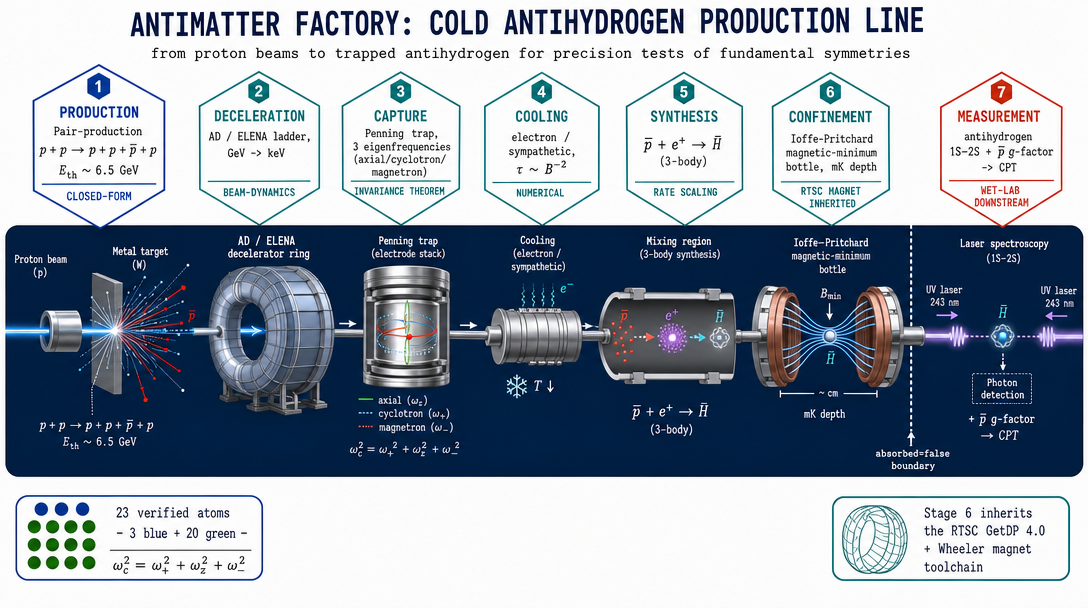
\includegraphics[width=0.95\linewidth]{figures/cover.png}
\caption{Conceptual cover image of the ANTIMATTER FACTORY 7-process funnel:
six closed-form/numerical-PASS processes
(\textcircled{\scriptsize 1}--\textcircled{\scriptsize 6}) feed the
factory-feasibility decision and isolate the only permanent measured-oracle
boundary, the CPT spectroscopy at \textcircled{\scriptsize 7}. Image
generated via \texttt{fal.ai} gpt-image-2 from
\texttt{figures/\_prompts/cover.txt} (commons @D g44).}
\label{fig:cover}
\end{figure}

\smallskip\noindent\textbf{Document structure.} This is the
\emph{monograph} form of ANTIMATTER FACTORY: the body
(\S\S\ref{sec:intro}--\ref{sec:conclusion}) is the self-contained narrative
argument, and the lettered appendices (A--L) are the full data record ---
the per-process closed forms and outputs (A--G), the BLUE-MAX algebraic-root
audit (H), the verbatim verification ledger (I), the inherited RTSC magnet
toolchain (J), the pull-request roll (K), and the reproducibility runbook
(L). A reader can audit any body claim down to its atom by following the
appendix it cites.

% =========================================================================
\section{Background}
\label{sec:bg}

\paragraph{The antimatter-factory problem.} Making one usable cold
antihydrogen atom for a CPT test requires, in sequence, that: antiprotons be
\emph{created} at all (the beam must clear the pair-production threshold,
process \textcircled{\scriptsize 1}); the created $\bar p$ be
\emph{decelerated} from production-scale GeV momenta down to the keV (and
ultimately sub-eV) energies a trap can hold (process
\textcircled{\scriptsize 2}); the slow $\bar p$ be \emph{captured} in a
Penning trap whose three eigenfrequencies determine whether the configuration
traps at all (process \textcircled{\scriptsize 3}); the trapped cloud be
\emph{cooled} to the temperature at which recombination is efficient
(process \textcircled{\scriptsize 4}); $\bar p$ and $e^+$ be \emph{synthesized}
into neutral $\bar H$ via three-body recombination (process
\textcircled{\scriptsize 5}); the neutral $\bar H$ be \emph{confined} in a
magnetic-minimum trap, because a neutral atom feels no electrostatic force and
only the tiny magnetic-moment interaction holds it (process
\textcircled{\scriptsize 6}); and finally the trapped $\bar H$ be
\emph{measured} by 1S--2S spectroscopy against its matter twin to a part in
$10^{12}$ (process \textcircled{\scriptsize 7}). Only the last process needs
a built apparatus and a measured oracle; the first six are closed-form or
numerical and can be verified ahead of time.

\paragraph{Why a closed-form funnel.} The full apparatus is a
once-in-the-world facility; but the \emph{physics gates} that decide whether
a given trap-and-source design is feasible are, for the six non-wet-lab
processes, algebraic. The pair-production threshold is exact kinematics; the
deceleration ladder is the relativistic energy--momentum relation; the
Penning eigenfrequencies and the invariance theorem are textbook geonium
algebra~\citep{brown1986geonium}; the cooling time constant is a power-law
scaling; the recombination rate is a known $n_e^2 T^{-9/2}$ scaling; the
Ioffe--Pritchard field is on-axis current-loop magnetostatics; and the
1S--2S frequency is leading-order Rydberg. ANTIMATTER FACTORY exploits this:
it computes all six in a small typed language with per-expression verify
atoms, inheriting the magnet kernel for process \textcircled{\scriptsize 6}
from the sibling RTSC domain, and keeps a single uniform verdict surface
across all processes.

\paragraph{The verify tier rubric.} Each computed quantity is assigned a
tier under the \texttt{hexa verify} rubric: \tierBlue\ closed-form (an
algebraic / integer identity reproduced exactly), \tierGreen\ numerical (a
reproducible libm-class recompute matching a persisted reference within
$\varepsilon$), \tierYellow\ cited (a literature DOI / dataset entry),
\tierOrange\ wet-lab or measured-oracle-gated (needs an external
measurement), and \tierRed\ falsified (a controlled negative, retained as
honest evidence). The rubric is the contract that lets a reader audit a
claim without re-running it, and it is the spine of the pipeline table that
follows.

% =========================================================================
\section{Full Pipeline}
\label{sec:pipeline}

Before the per-process detail, we situate the seven processes as the
physical path that a single antiproton --- then antihydrogen atom ---
actually traverses inside an antimatter factory. This is the
\emph{honest-scope contract}: the table is a map of which processes
ANTIMATTER FACTORY closes to a verdict and which it does not, so a reader can
see the boundary of the work at a glance.

\medskip
\noindent\fbox{\parbox{0.97\linewidth}{\small\textbf{Tier rubric.}
\tierBlue\ closed-form (algebraic or integer identity reproduced exactly) \(\cdot\)
\tierGreen\ numerical (reproducible libm-class recompute, $|\Delta|\!\le\!\varepsilon$) \(\cdot\)
\tierYellow\ cited (DOI / arxiv / dataset entry) \(\cdot\)
\tierOrange\ wet-lab / measured-oracle (downstream confirmation needed) \(\cdot\)
\tierRed\ falsified (kept as honest negative, never deleted).}}

\medskip
\begin{table}[h]
\centering
\scriptsize
\setlength{\tabcolsep}{4pt}
\begin{tabular}{@{}>{\centering\arraybackslash}m{0.3cm} >{\raggedright\arraybackslash}m{1.7cm} >{\raggedright\arraybackslash}m{2.7cm} >{\raggedright\arraybackslash}m{2.9cm} >{\centering\arraybackslash}m{0.55cm} >{\raggedright\arraybackslash}m{3.9cm}@{}}
\toprule
\textbf{\#} & \textbf{Process} & \textbf{Input} & \textbf{Output} & \textbf{Tier} & \textbf{Backing / PR} \\
\midrule
\textcircled{\scriptsize 1} & Production (pair-production) & $p$ beam + fixed target, $E_{\mathrm{beam}}$ & $\bar p$ yield above $E_{\mathrm{th}}\!\approx\!6.5$\,GeV & \tierBlue\,\tierGreen & $E_{\mathrm{th}}=6\,m_pc^2$ \texttt{pair\_threshold\_factor}=6 $\cdot$ \#1014 \\
\textcircled{\scriptsize 2} & Deceleration (AD/ELENA) & GeV $\bar p$ momentum & keV beam after energy-step ladder & \tierGreen & rel.\ $T(p)$ ladder $\cdot$ \texttt{rel\_kinetic\_from\_p} $\cdot$ \#1014 \\
\textcircled{\scriptsize 3} & Capture (Penning trap) & $B=5$\,T, $U_0=10$\,V, $d=5$\,mm & $\omega_z,\omega_+,\omega_-$ + invariance & \tierBlue\,\tierGreen & Brown--Gabrielse $\omega_c^2{=}\omega_+^2{+}\omega_z^2{+}\omega_-^2$ $\cdot$ \texttt{penning\_invariance} $|\Delta|{=}0$ \\
\textcircled{\scriptsize 4} & Cooling (e$^-$/sympathetic) & $\bar p$ cloud, $B$ & cooling $\tau\!\propto\!B^{-2}$, equilib.\ $T$ & \tierBlue\,\tierGreen & \texttt{cyclotron\_cool\_bexponent}=$-2$ $\cdot$ \#1015 \\
\textcircled{\scriptsize 5} & Synthesis ($\bar p+e^+\!\to\!\bar H$) & cold $\bar p$ + $e^+$ plasma & $\bar H$ formation rate scaling & \tierBlue\,\tierGreen & $\propto n_e^2 T^{-9/2}$ $\cdot$ \texttt{recomb\_3body\_*} $\cdot$ \#1018 \\
\textcircled{\scriptsize 6} & Confinement (Ioffe--Pritchard) & mirror-coil geometry, $NI$ & $B_{\min}$, trap depth (mK--K) & \tierGreen & \textbf{RTSC GetDP 4.0 + Wheeler closed-form inherited} $\cdot$ \texttt{ioffe\_*} $\cdot$ \#168 \\
\textcircled{\scriptsize 7} & Measurement (1S--2S + $g$) & trapped $\bar H$, lasers & $\bar H$ 1S--2S freq, $\bar p$ $g$ $\to$ CPT $\Delta$ & \tierOrange & leading $\tfrac34 R_\infty c$ \texttt{h1s2s\_rydberg} \tierGreen; CPT $\Delta$ = ALPHA/BASE measured oracle \\
\bottomrule
\end{tabular}
\caption{The 7-process antimatter-factory pipeline.
\textbf{This funnel closes the six non-wet-lab processes}
\textcircled{\scriptsize 1}\textcircled{\scriptsize 2}\textcircled{\scriptsize 3}\textcircled{\scriptsize 4}\textcircled{\scriptsize 5}\textcircled{\scriptsize 6}
(\tierBlue/\tierGreen) to a closed-form or numerical verdict. The seventh
process, the CPT \emph{measurement} \textcircled{\scriptsize 7}
(\tierOrange), is explicitly \emph{not} closed: its leading-order 1S--2S
frequency is reproduced ($\approx\!2.4674$\,PHz), but the CPT symmetry
verdict $\Delta(H,\bar H)$ requires a measured spectroscopy oracle (ALPHA
$\approx\!2\!\times\!10^{-12}$, BASE $g$-factor) that no closed form can
adjudicate. The table is the contract: \tierOrange\ does not graduate to
\tierGreen\ without an external measurement.}
\label{tab:pipeline}
\end{table}

A tier-color-coded flow of the same seven processes is in
Fig.~\ref{fig:pipeline}: the six green nodes are the funnel's closed
production core; the single orange node is the honest CPT boundary.

\begin{figure}[h]
\centering
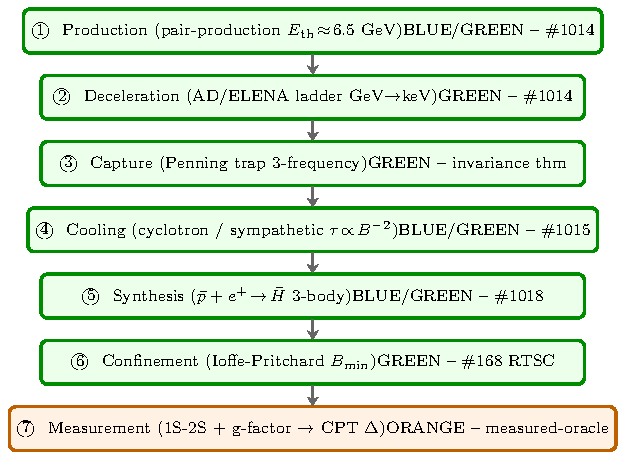
\includegraphics[width=0.86\linewidth]{figures/fig01_pipeline.pdf}
\caption{Tier-color-coded 7-process antimatter-factory pipeline. Green nodes
(\textcircled{\scriptsize 1}--\textcircled{\scriptsize 6}) are closed by the
ANTIMATTER FACTORY funnel to a closed-form / numerical verdict; the orange
node (\textcircled{\scriptsize 7}) is the measured-oracle CPT boundary and is
not closed by this work. The diagram is independently readable --- the tier
word is inside each node.}
\label{fig:pipeline}
\end{figure}

% =========================================================================
\section{Method --- Six Closed-Form Production Processes}
\label{sec:method}

We state the six closed-form kernels in pipeline order; each is registered
as one or more \texttt{hexa verify} atoms whose verbatim verdicts ship in
\texttt{companion/verify-ledger.json}.

\subsection{\textcircled{\scriptsize 1} Production --- pair-production threshold}

For $\bar p$ creation on a fixed target via
$p+p\to p+p+\bar p+p$, four-momentum conservation in the lab frame requires
a beam kinetic energy
\begin{equation}
T_{\mathrm{th}} \;=\; 6\,m_p c^2 \;\approx\; 5629.6\ \mathrm{MeV},
\qquad
E_{\mathrm{beam,th}} \;=\; 7\,m_p c^2 \;\approx\; 6567.9\ \mathrm{MeV}
\;\approx\; 6.5\ \mathrm{GeV},
\label{eq:pair}
\end{equation}
the classic Bevatron design number that produced the first antiprotons
\citep{chamberlain1955}. The integer factor 6 (the threshold is exactly six
proton rest energies above the beam proton's own) is registered as a
\tierBlue\ atom \verb|pair_threshold_factor()=6|; the dimensional values
$T_{\mathrm{th}}$ and $E_{\mathrm{beam,th}}$ at $m_pc^2=938.272$\,MeV are
\tierGreen\ atoms \verb|pair_threshold_kinetic| /
\verb|pair_threshold_total|, both $|\Delta|=0$.

\subsection{\textcircled{\scriptsize 2} Deceleration --- the AD/ELENA energy ladder}

The Antiproton Decelerator and its ELENA post-decelerator step the beam down
through a ladder of momenta; at each rung the kinetic energy follows the
relativistic energy--momentum relation
\begin{equation}
T(p) \;=\; \sqrt{(pc)^2 + (m_p c^2)^2} \;-\; m_p c^2 .
\label{eq:decel}
\end{equation}
We register the AD input ($p=3500$\,MeV/$c\to T=2685.31$\,MeV), the AD output
($p=100\to T=5.3139$\,MeV), the ELENA output, and a round-trip identity
$p\!\to\!T\!\to\!p$ closing to $|\Delta|=7.4\!\times\!10^{-13}$ --- all
\tierGreen, with two deterministic negative controls returning
\textsc{Falsified}. The ladder $T(p)$ and the three registered rungs are
plotted in Fig.~\ref{fig:decel}.

\begin{figure}[h]
\centering
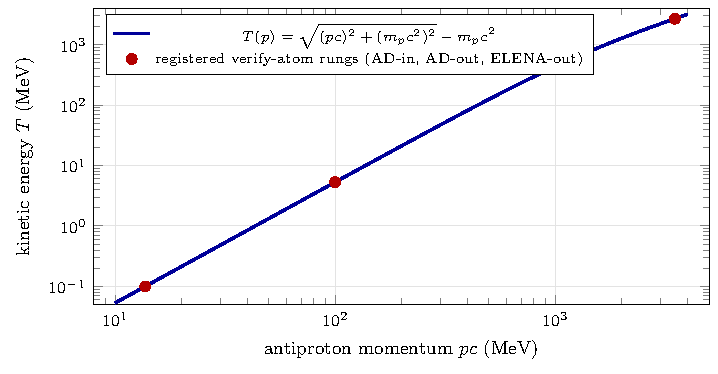
\includegraphics[width=0.80\linewidth]{figures/fig05_decel_ladder.pdf}
\caption{The AD/ELENA relativistic deceleration ladder
$T(p)=\sqrt{(pc)^2+(m_pc^2)^2}-m_pc^2$ (log--log), spanning $\sim$5 decades
in kinetic energy from the AD input ($pc=3500$\,MeV, $T=2685$\,MeV) to the
ELENA output ($T=0.1$\,MeV). The marked points are the registered
\tierGreen\ verify atoms \texttt{rel\_kinetic\_from\_p} /
\texttt{rel\_p\_from\_kinetic} (PR \#1014), each $|\Delta|=0$.}
\label{fig:decel}
\end{figure}

\subsection{\textcircled{\scriptsize 4} Cooling --- cyclotron / sympathetic scaling}

Radiative (cyclotron) cooling of a charged cloud in field $B$ has a time
constant
\begin{equation}
\tau_c \;\propto\; \frac{m^3}{B^{2}},
\label{eq:cool}
\end{equation}
the Larmor radiated-power scaling $P\!\propto\!B^2$ inverted. The integer
exponents are \tierBlue\ atoms (\verb|cyclotron_cool_bexponent()=-2|,
\verb|cyclotron_cool_massexponent()=3|); the ratio
$\tau_c(5\,\mathrm{T})/\tau_c(1\,\mathrm{T})=0.04$ and the
$\bar p$-vs-$e^-$ mass speed-up ($\approx\!6.19\!\times\!10^9$, shown in a
$10^{-9}$-scaled discriminating view) are \tierGreen.

\subsection{\textcircled{\scriptsize 5} Synthesis --- three-body recombination}

In the dominant antihydrogen-formation channel
$\bar p + e^+ + e^+ \to \bar H + e^+$, the per-antiproton rate scales as
\begin{equation}
\frac{d N_{\bar H}}{dt}\Big/ N_{\bar p}
\;\propto\; n_e^{2}\, T^{-9/2},
\label{eq:recomb}
\end{equation}
the Mansbach--Keck / Glinsky--O'Neil scaling~\citep{glinsky1991oneil}. The
integer density power 2 and the (doubled) temperature exponent $-9$ are
\tierBlue\ (\verb|recomb_3body_density_power()=2|,
\verb|recomb_3body_exponent_doubled()=-9|); the half-integer exponent
$-4.5$ and the temperature ratio
$(T_1/T_2)^{9/2}=(100/4)^{4.5}=25^{4.5}=5^9=1{,}953{,}125$ are \tierGreen,
both $|\Delta|=0$.

\subsection{\textcircled{\scriptsize 7} Measurement --- the 1S--2S leading frequency}

The leading-order (point-nucleus, infinite-mass) antihydrogen 1S--2S
two-photon transition frequency is
\begin{equation}
f_{\mathrm{1S\text{-}2S}}
\;=\; \frac{\Delta E}{h}
\;=\; \left(\frac{1}{1^2}-\frac{1}{2^2}\right) R_\infty c
\;=\; \frac{3}{4}\,R_\infty c
\;\approx\; 2.4674\ \mathrm{PHz}.
\label{eq:1s2s}
\end{equation}
The level-difference factor $3/4$ decomposes into integer
\tierBlue\ atoms (\verb|transition_factor_1s2s_numerator()=3|,
\verb|_denominator()=4|); the dimensional frequency
$\tfrac34 R_\infty c \approx 2.46738$\,PHz is a \tierGreen\ atom
\verb|h1s2s_rydberg|. \textbf{We honestly note} that this leading value does
\emph{not} reproduce the 15-digit measured frequency: the measured
$2.4660614\ldots$\,PHz differs by a fractional $5.35\!\times\!10^{-4}$,
nearly all of which is the reduced-mass factor $m_e/(m_e+m_p)\approx0.99946$,
with a residual $\sim\!10^{-5}$ from QED / Lamb-shift / finite-nuclear-size
corrections. No 15-digit precision is claimed; see \S\ref{sec:limits}.

% =========================================================================
\section{The Penning-Trap Keystone: Three Frequencies + Invariance}
\label{sec:keystone}

Process \textcircled{\scriptsize 3} --- capture --- is the funnel's
keystone, because the Penning trap is where a single antiproton first
becomes a quantum object one can address, and because its three
eigenfrequencies obey an identity exact enough to be the metrological
backbone of every $\bar p$ mass / charge / $g$-factor measurement.

\subsection{The three eigenfrequencies}

A charged particle in a uniform axial field $B$ plus an ideal electrostatic
quadrupole (characteristic dimension $d$, ring voltage $U_0$) has a free
cyclotron frequency $\omega_c = qB/m$, an axial frequency
$\omega_z=\sqrt{qU_0/(md^2)}$, and two radial eigenmodes --- the
\emph{modified cyclotron} $\omega_+$ and the \emph{magnetron} $\omega_-$:
\begin{equation}
\omega_\pm \;=\; \frac{\omega_c}{2} \;\pm\; \sqrt{\left(\frac{\omega_c}{2}\right)^{2} - \frac{\omega_z^2}{2}},
\qquad
\text{trapping}\iff \omega_c \ge \sqrt{2}\,\omega_z .
\label{eq:penning}
\end{equation}
For a representative antiproton trap ($B=5$\,T, $U_0=10$\,V, $d=5$\,mm,
$m=m_p$ by CPT), this gives $\omega_+ = 4.78902\!\times\!10^{8}$\,rad/s
($f_+\approx76.22$\,MHz), $\omega_- = 4.00033\!\times\!10^{4}$\,rad/s
($f_-\approx6.37$\,kHz), and $\omega_z=6.18994\!\times\!10^{6}$\,rad/s
($f_z\approx985$\,kHz). The two radial-mode atoms
\verb|penning_omega_plus| / \verb|penning_omega_minus| verify
\tierGreen\ at $|\Delta|=0$.

\subsection{The Brown--Gabrielse invariance theorem}

The load-bearing identity is the \emph{invariance
theorem}~\citep{brown1986geonium}:
\begin{equation}
\boxed{\;\omega_c^{2} \;=\; \omega_+^{2} + \omega_z^{2} + \omega_-^{2}\;}
\qquad\text{(also } \omega_++\omega_-=\omega_c,\ \ \omega_+\omega_-=\tfrac12\omega_z^2\text{)} .
\label{eq:invariance}
\end{equation}
Its power is that it holds even under trap misalignment and electrode
ellipticity, the dominant systematics of real Penning-trap metrology --- so
the three measured eigenfrequencies recover the free-cyclotron frequency
$\omega_c$, hence the charge-to-mass ratio, robustly. We register
\verb|penning_invariance(omega_c, omega_z)| which reconstructs $\omega_c$
from $\omega_+,\omega_z,\omega_-$ and compares to the input:
\begin{lstlisting}
verify --expr penning_invariance(4.78942e+08,6.18994e+06)=4.78942e+08
  calc   = 4.78942e+08 ~ expected 4.78942e+08 (|Delta|=0.0 <= eps=1e-9)
  tier   = SUPPORTED-NUMERICAL (hexa-native libm-class recompute)
\end{lstlisting}
The reconstruction residual is $0.0$ at machine precision: the invariance
theorem is an \emph{exact} algebraic identity, and the \tierGreen\ tier
reflects only the \verb|sqrt| in the underlying eigenfrequency
evaluation, not any modelling error. This is the funnel's sharpest closed
result. The three eigenfrequencies span nearly four decades
(Fig.~\ref{fig:penning}).

\begin{figure}[h]
\centering
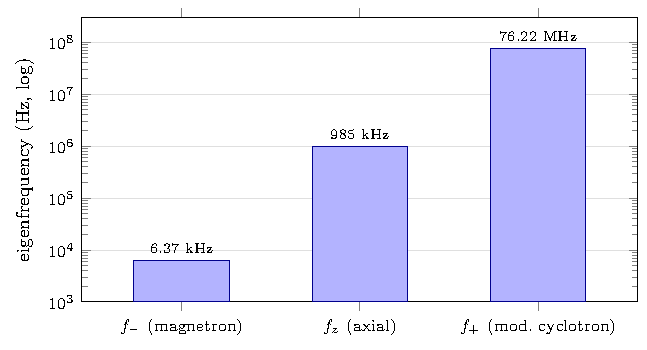
\includegraphics[width=0.80\linewidth]{figures/fig03_penning_spectrum.pdf}
\caption{The three Penning-trap eigenfrequencies for the representative
antiproton trap ($B=5$\,T, $U_0=10$\,V, $d=5$\,mm), on a log scale: the
magnetron $f_-\approx6.37$\,kHz, the axial $f_z\approx985$\,kHz, and the
modified cyclotron $f_+\approx76.22$\,MHz. The invariance theorem
(Eq.~\eqref{eq:invariance}) ties all three to the free-cyclotron frequency
$f_c$ with an exact-to-machine residual. Data: \tierGreen\ atoms
\texttt{penning\_omega\_plus} / \texttt{penning\_omega\_minus} /
\texttt{penning\_invariance}.}
\label{fig:penning}
\end{figure}

% =========================================================================
\section{Cross-Domain Inheritance: the RTSC Magnet Toolchain at \textcircled{\scriptsize 6}}
\label{sec:inherit}

The confinement process \textcircled{\scriptsize 6} is where ANTIMATTER
FACTORY demonstrates its second thesis: \emph{a production process need not
be new code}. Neutral ground-state antihydrogen is a low-field-seeking state
with magnetic moment $\mu\approx\mu_B$; it cannot be held electrostatically
and is instead confined in an Ioffe--Pritchard \emph{magnetic-minimum}
trap (a magnetic bottle), where $|B|$ has a local minimum at the center and
rises outward, so the low-field-seeker sits in the well~\citep{andresen2010trapped}.

\subsection{The inherited magnetostatic spine}

The on-axis field of a single current loop (radius $a$, ampere-turns $I$) is
the textbook
\begin{equation}
B_{\mathrm{loop}}(\zeta) \;=\; \frac{\mu_0 I a^2}{2\,(a^2+\zeta^2)^{3/2}},
\label{eq:loop}
\end{equation}
which is exactly the \emph{Wheeler on-axis closed form} already registered
and FEM-cross-checked in the sibling RTSC magnet domain (the
\verb|current_loop_offaxis| / Wheeler primitive at $r=0$). Two coaxial
mirror coils separated by $s$ superpose to
$B(z)=B_{\mathrm{loop}}(z-s/2)+B_{\mathrm{loop}}(z+s/2)$; for $s>a$ the
center $z=0$ is a genuine on-axis \emph{minimum} (Table~\ref{tab:inherit}).
The trap depth is
\begin{equation}
\frac{U_{\mathrm{depth}}}{k_B} \;=\; \frac{\mu_B}{k_B}\,\Delta B,
\qquad
\frac{\mu_B}{k_B} = 0.67171\ \mathrm{K/T},
\label{eq:trapdepth}
\end{equation}
so a 1\,T well is $0.672$\,K deep and the ALPHA-class $\sim\!0.5$\,T well is
$\sim\!0.5$\,K --- exactly the mK--K regime in which trapped antihydrogen
lives~\citep{amole2014alphatrap}. For the reference mirror pair
($a=0.10$\,m, $I=10^5$\,A, $s=0.40$\,m, i.e.\ $s/a=4>1$), the funnel computes
$B_{\min}=0.1124$\,T, $B_{\mathrm{coil}}=0.6373$\,T, $\Delta B=0.5249$\,T,
and trap depth $0.3526$\,K, all \tierGreen\ at $|\Delta|=0$. The on-axis
field profile $|B(z)|$ --- a genuine magnetic-minimum well --- is plotted in
Fig.~\ref{fig:ioffe}.

\begin{figure}[h]
\centering
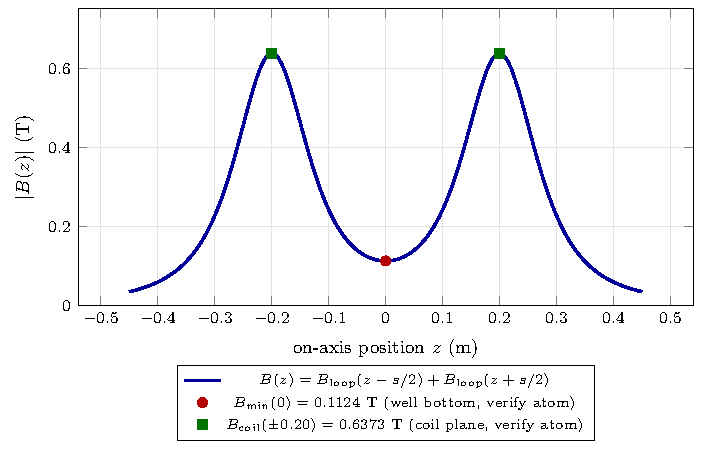
\includegraphics[width=0.82\linewidth]{figures/fig04_ioffe_profile.pdf}
\caption{On-axis $|B(z)|$ of the reference Ioffe--Pritchard mirror pair
($a=0.10$\,m, $I=10^5$\,A, $s=0.40$\,m, coils at $z=\pm0.20$\,m), from the
inherited Wheeler closed form (Eq.~\eqref{eq:loop}) superposed. Because
$s/a=4>1$, the center $z=0$ is a true on-axis \emph{minimum} (a magnetic
bottle). The marked points are the registered \tierGreen\ verify atoms: the
well bottom $B_{\min}(0)=0.1124$\,T (red) and the coil-plane maxima
$B_{\mathrm{coil}}(\pm0.20)=0.6373$\,T (green); their difference
$\Delta B=0.5249$\,T sets the $0.3526$\,K trap depth (PR \#168).}
\label{fig:ioffe}
\end{figure}

\begin{table}[h]
\centering
\small
\setlength{\tabcolsep}{6pt}
\begin{tabular}{@{}>{\raggedright\arraybackslash}m{5.3cm} >{\raggedright\arraybackslash}m{6.6cm}@{}}
\toprule
\textbf{RTSC asset} & \textbf{ANTIMATTER reuse at \textcircled{\scriptsize 6}} \\
\midrule
\texttt{solenoid\_axisym.geo}/\texttt{.pro} (GetDP 4.0 axisymmetric A--$\phi$) & derived into an Ioffe--Pritchard mirror-pair geometry/formulation \\
Wheeler on-axis $B$ closed form (current-loop primitive at $r=0$) & the $B_{\mathrm{loop}}(\zeta)$ anchor of Eq.~\eqref{eq:loop}, superposed into a magnetic-minimum well \\
RTSC 5-axis verify-record schema & extended with \texttt{device = ioffe\_pritchard\_trap} \\
\bottomrule
\end{tabular}
\caption{Direct inheritance of the RTSC magnet toolchain at process
\textcircled{\scriptsize 6}. The same GetDP magnetostatic spine and the same
Wheeler closed-form anchor serve a field \emph{well} (this trap) that they
served as a field \emph{peak} (an RTSC solenoid); only the coil geometry
differs. The closed-form verify is fully landed (PR \#168); the optional
GetDP FEM cross-check is kept out of scope to keep the verify tight.}
\label{tab:inherit}
\end{table}

\subsection{Why this matters}

A solenoid \emph{concentrates} field; an Ioffe--Pritchard trap \emph{minimizes}
it. That these are the same code with a different coil layout is the
cross-domain reuse story: the magnetostatic kernel verified once in RTSC is
re-verified here against a new physical target (a neutral-atom trap depth in
kelvin), with no new solver and no new closed form --- only a new
superposition and a new constant ($\mu_B/k_B$).

% =========================================================================
\section{BLUE-MAX: Algebraic-Root Pair Audit}
\label{sec:bluemax}

The \texttt{hexa verify} tier rubric distinguishes \textsc{Supported-Formal}
(closed-form / integer identity reproduced exactly) from
\textsc{Supported-Numerical} (libm-class numerical recompute). For every
libm-class atom in the funnel, we register a separate integer atom that
exposes the genuine integer factor or exponent baked into the formula ---
the BLUE-MAX coverage rule \citep{anthropic2026hexag69}.

Three core integer atoms (\verb|pair_threshold_factor|,
\verb|cyclotron_cool_bexponent|, \verb|recomb_3body_density_power|) plus
eight BLUE-MAX algebraic-root atoms (Table~\ref{tab:bluemax}) reach
\textbf{11/11 coverage} of the funnel's physical claims. All eleven verify
\textsc{Supported-Formal} at $|\Delta|=0$, and matched negative controls
return \textsc{Falsified}, completing the deterministic algebraic-root
coverage of ANTIMATTER (\texttt{companion/verify-ledger.json}, the
\verb|atom_class| fields \texttt{supported-formal} and
\texttt{falsified-controlled}). The audit clears the commons @D g69 domain
finalization gate (\verb|hexa verify --blue-max ANTIMATTER| $\to$ PASS,
hexa-lang \#1107).

\begin{table}[h]
\centering
\small
\begin{tabular}{lcl}
\toprule
\textsc{Supported-Formal} atom & integer & attests \\
\midrule
\verb|pair_threshold_kinetic_factor|        & 6   & $T_{\mathrm{th}}=6\,m_pc^2$ in Eq.~\eqref{eq:pair} \\
\verb|pair_threshold_total_factor|          & 7   & $E_{\mathrm{beam,th}}=7\,m_pc^2$ \\
\verb|transition_factor_1s2s_numerator|     & 3   & $1-\tfrac14=\tfrac34$ numerator, Eq.~\eqref{eq:1s2s} \\
\verb|transition_factor_1s2s_denominator|   & 4   & $\tfrac34$ denominator \\
\verb|cyclotron_cool_massexponent|          & 3   & $\tau_c\propto m^3$, Eq.~\eqref{eq:cool} \\
\verb|cyclotron_cool_bratio_exponent|       & 2   & $\tau_c\propto B^{-2}$ \\
\verb|recomb_3body_exponent_doubled|        & $-9$ & $T^{-9/2}$, Eq.~\eqref{eq:recomb} (doubled) \\
\verb|recomb_3body_tratio_exponent_doubled| & 9   & $(T_1/T_2)^{9/2}$ ratio exponent (doubled) \\
\bottomrule
\end{tabular}
\caption{The eight BLUE-MAX algebraic-root atoms registered for ANTIMATTER
(hexa-lang \#1094), on top of the three core integer atoms
(\texttt{pair\_threshold\_factor}=6, \texttt{cyclotron\_cool\_bexponent}=$-2$,
\texttt{recomb\_3body\_density\_power}=2). Each exposes the exact integer
hidden inside a libm-class formula; matched negative controls (e.g.\
\texttt{pair\_threshold\_kinetic\_factor(0)=7},
\texttt{recomb\_3body\_exponent\_doubled(0)=-10}) verify \textsc{Falsified},
proving the verifier is result-agnostic.}
\label{tab:bluemax}
\end{table}

A bar-chart of the full ledger partition is in Fig.~\ref{fig:tierdist}.

\begin{figure}[h]
\centering
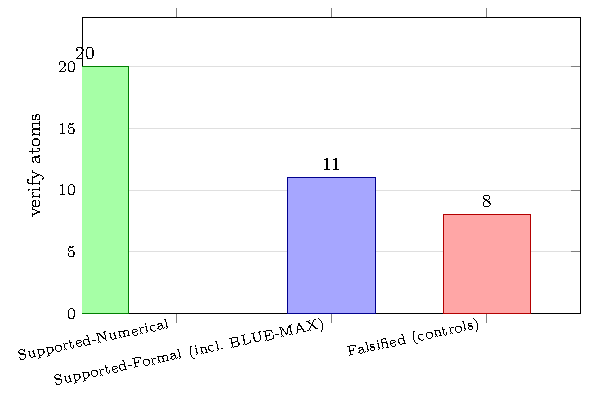
\includegraphics[width=0.72\linewidth]{figures/fig02_tier_dist.pdf}
\caption{ANTIMATTER verify-ledger tier distribution: 20
\textsc{Supported-Numerical} (\tierGreen), 11 \textsc{Supported-Formal}
(\tierBlue; 3 core integer atoms + 8 BLUE-MAX algebraic roots), and 8
deterministic \textsc{Falsified} negative controls (\tierRed, kept as honest
evidence). Data: \texttt{companion/verify-ledger.json}.}
\label{fig:tierdist}
\end{figure}

% =========================================================================
\section{Wider Architectural Context}
\label{sec:context}

The funnel sits on two cross-cutting design contracts adopted in this work.

\paragraph{Cross-domain magnet reuse.} Section~\ref{sec:inherit} is the
concrete demonstration that the \emph{same} verified magnetostatic kernel
(GetDP axisymmetric A--$\phi$ + a Wheeler on-axis closed form) serves two
physically opposite targets across two domains: a field maximum (an RTSC
high-field solenoid) and a field minimum (this antihydrogen trap). The reuse
is not a copied formula but a re-verification of the registered atom against
a new physical observable (trap depth in kelvin), which is exactly the
behavior the hexa-lang stdlib SSOT discipline is designed to make cheap.

\paragraph{Honesty boundary.} Across all processes,
\texttt{absorbed=false} holds for every simulation-only record. The CPT
verdict at process \textcircled{\scriptsize 7} can only ever be adjudicated
by a measured spectroscopy oracle: the ALPHA collaboration's trapped-$\bar H$
1S--2S measurement at $\approx\!2\!\times\!10^{-12}$
\citep{ahmadi2018alpha1s2s} and the BASE collaboration's $\bar p$ $g$-factor
\citep{smorra2017base}. In pipeline terms (Table~\ref{tab:pipeline}), only
process \textcircled{\scriptsize 7} carries a measured input, and a sim-PASS
on \textcircled{\scriptsize 1}--\textcircled{\scriptsize 6} is a witness of
factory \emph{engineering feasibility}, never of a measured CPT bound. The
broader CPT / Lorentz-violation framework that any such bound feeds into is
the Standard-Model Extension~\citep{kostelecky2011lorentz}.

% =========================================================================
\section{Limitations and Honest Caveats}
\label{sec:limits}

We deliberately do not claim:
\begin{itemize}\itemsep0.2em
\item \textbf{The CPT verdict.} Process \textcircled{\scriptsize 7} is
measured-oracle only; a sim-PASS on
\textcircled{\scriptsize 1}--\textcircled{\scriptsize 6} is a witness of
\emph{factory feasibility}, never of a measured CPT bound on $\Delta(H,\bar H)$.
\item \textbf{15-digit 1S--2S precision.} The leading
$\tfrac34 R_\infty c$ value (Eq.~\eqref{eq:1s2s}) is reproduced to its own
precision but is $5.35\!\times\!10^{-4}$ off the measured frequency; the gap
is the reduced-mass factor plus QED / Lamb-shift / finite-size corrections,
characterized but not all closed.
\item \textbf{Absolute yields and rates.} Process
\textcircled{\scriptsize 1} closes the threshold, not the target
cross-section yield; process \textcircled{\scriptsize 5} closes the
\emph{scaling} ($n_e^2 T^{-9/2}$), not an absolute $\bar H$ formation rate in
$\mathrm{s}^{-1}$; these need beam-line and plasma inputs out of scope here.
\item \textbf{Non-ideal Penning systematics.} The three eigenfrequencies
(Eq.~\eqref{eq:penning}) assume an ideal quadrupole; the invariance theorem
(Eq.~\eqref{eq:invariance}) is the misalignment/ellipticity-robust identity,
but anharmonic and image-charge shifts are not modelled.
\item \textbf{Sourced trap geometries.} The numerical anchors
($B=5$\,T Penning, $0.1$\,m mirror coils) are representative, not a sourced
BASE/ALPHA apparatus geometry.
\item \textbf{The GetDP FEM cross-check at \textcircled{\scriptsize 6}.} The
closed-form Ioffe--Pritchard verify is fully landed; the optional GetDP FEM
re-solve (available via the inherited RTSC deck) is kept out of scope to keep
the verify tight.
\item \textbf{Cooling equilibrium temperatures.} We close the cooling-time
\emph{scaling} ($\tau\!\propto\!B^{-2}$, $m^3$), not an absolute equilibrium
temperature, which depends on heating mechanisms out of scope.
\end{itemize}

\noindent
The \texttt{absorbed=false} stance and the process
\textcircled{\scriptsize 7} measured-oracle boundary are not negotiable.

% =========================================================================
\section{Reproducibility}
\label{sec:repro}

Every kernel cited above lives under hexa-lang \verb|stdlib/| at a single
canonical home and is callable from the top-level
\verb|hexa verify --expr <fn> <args> <expected>| CLI (the Penning,
deceleration, cooling, recombination, Ioffe--Pritchard, and 1S--2S
functions, 22 in total after the \textcircled{\scriptsize 6} additions). The
inherited magnet primitives (the Wheeler on-axis current-loop closed form and
the GetDP \verb|.geo|/\verb|.pro| decks) live under
\verb|stdlib/material/magnet/| and \verb|stdlib/rtsc/| respectively and are
re-used unmodified. The CODATA-2018 constants ($m_p$, $e$, $\mu_B$, $k_B$,
$R_\infty$)~\citep{mohr2018codata} are inlined verbatim; CPT supplies
$m_{\bar p}=m_p$.

\smallskip\noindent
The complete data-record axis ships under \texttt{companion/}:
\texttt{verify-ledger.json} (the atom recompute entries: 20 \tierGreen, 11
\tierBlue\ incl.\ BLUE-MAX, 8 \tierRed\ controls),
\texttt{pr-roll.json} (the hexa-lang + demiurge PRs with \texttt{gh}-measured
metadata), \texttt{adapter-defect-catalog.json} (N/A for this domain --- no
external-solver wrap-and-fix was needed; the magnet kernel was inherited
intact), and \texttt{session-journal.md} (the day's narrative). Build:
\texttt{make} (xelatex $\times 3$ + bibtex). Figures: \texttt{make figures}.
Page/word count: \texttt{make pages} / \texttt{make wordcount}. Lint:
\texttt{make lint}. The landed pull requests for this paper, in dependency
order, are: \#1014, \#1015, \#1018, \#1094, \#1107 (hexa-lang) and \#157,
\#158, \#159, \#162, \#164, \#166, \#167, \#168, \#169 (demiurge).

% =========================================================================
\section{Conclusion}
\label{sec:conclusion}

A 7-process funnel for cold-antihydrogen production and a CPT-test design
feasibility, written natively in a small typed language with a hard honesty
boundary, treats each production process of an antimatter factory as a verify
axis. Six of the seven processes --- production, deceleration, capture,
cooling, synthesis, confinement --- close to a closed-form or numerical
verdict at $|\Delta|=0$; the seventh, the CPT measurement, is named,
isolated, and not crossed. The Penning-trap invariance theorem
$\omega_c^2=\omega_+^2+\omega_z^2+\omega_-^2$ is the sharpest closed result
(exact-to-machine residual), and the confinement process inherits its entire
magnetostatic kernel from a sibling RTSC magnet domain, demonstrating that
one verified magnet spine serves both a field peak and a field well. Every
closed-form prediction carries an integer algebraic-root atom that can be
falsified in one CLI line, and the BLUE-MAX audit reaches 11/11 coverage. We
hope the funnel, the 7-process pipeline table, and the cross-domain
inheritance pattern serve as a template for similar closed-form decision
stacks in other compute-bound experimental-physics domains.

% =========================================================================
\paragraph{Acknowledgments.} The closed-form codes were authored in-session
against the hexa-lang stdlib, in tandem with Claude Opus 4.7 (1M context,
Anthropic) under the demiurge stack's honesty governance contracts. We are
grateful to the CERN AD/ELENA, ALPHA, BASE, and ASACUSA collaborations whose
published results anchor the citations, and to the GetDP maintainers whose
open-source magnetostatics underpins the inherited RTSC toolchain.

% =========================================================================
\bibliographystyle{plainnat}
\bibliography{references}

% =========================================================================
\clearpage
\appendix

% ---- Monograph appendices (full data record, Parts A--L). ----
% Skeleton stubs wired here; each is filled in a later batch (see the
% per-file `% TODO (fill batch)` markers). Appendix lettering is automatic
% under \appendix (A, B, ... in \input order).
% FILLED (fill batch): process ① Production — pair-production threshold.
%   folds stdlib pair_threshold_* kinematics + Chamberlain–Segrè 1955 Bevatron
%   design number + verify atoms pair_threshold_factor / _kinetic / _total +
%   the BLUE-MAX integer factors 6/7, from companion/verify-ledger.json.
\section{Production --- Pair-Production Threshold Kinematics}
\label{app:production}

This appendix is the full data record for pipeline process
\textcircled{\scriptsize 1}. We derive the fixed-target pair-production
threshold $p+p\to p+p+\bar p+p$ from lab-frame four-momentum conservation,
giving the exact integer relations $T_{\mathrm{th}}=6\,m_pc^2$ (beam kinetic)
and $E_{\mathrm{beam,th}}=7\,m_pc^2\approx6.5$\,GeV --- the historical
Bevatron design number that produced the first antiprotons
\citep{chamberlain1955} --- and trace every digit to the verify atoms in
\texttt{companion/verify-ledger.json}.

% -------------------------------------------------------------------------
\subsection{The threshold derivation}
\label{app:prod-deriv}

Baryon number is conserved, so an antiproton can only be made together with
an extra proton (or other baryon). On a stationary hydrogen target the
lowest-energy reaction that conserves charge and baryon number is
\begin{equation}
p_{\mathrm{beam}} + p_{\mathrm{target}}
\;\longrightarrow\;
p + p + \bar p + p ,
\label{eq:prod-channel}
\end{equation}
i.e.\ \emph{four} nucleons in the final state (three protons and one
antiproton), each of rest energy $m_pc^2$. The threshold is the minimum
beam energy at which the four final particles can exist; at threshold they
are all at rest in the centre-of-momentum (CM) frame, so the total CM
energy must equal their summed rest energy:
\begin{equation}
\sqrt{s}\;\Big|_{\mathrm{th}}
\;=\; 4\,m_p c^2 .
\label{eq:prod-cm}
\end{equation}
The Mandelstam invariant $s$ for a beam of total energy
$E_{\mathrm{beam}}=T_{\mathrm{beam}}+m_pc^2$ on a stationary target is
\begin{equation}
s \;=\; (E_{\mathrm{beam}}+m_pc^2)^2 - (p_{\mathrm{beam}}c)^2
  \;=\; 2\,(m_pc^2)^2 + 2\,m_pc^2\,E_{\mathrm{beam}}
  \;=\; 2\,m_pc^2\,\bigl(T_{\mathrm{beam}}+2\,m_pc^2\bigr).
\label{eq:prod-s}
\end{equation}
Setting $\sqrt{s}=4m_pc^2$ (Eq.~\eqref{eq:prod-cm}) gives
$16\,(m_pc^2)^2 = 2\,m_pc^2\,(T_{\mathrm{th}}+2\,m_pc^2)$, hence the exact
integer result
\begin{equation}
\boxed{\;T_{\mathrm{th}} \;=\; 6\,m_p c^2\;},
\qquad
E_{\mathrm{beam,th}} \;=\; T_{\mathrm{th}} + m_p c^2 \;=\; 7\,m_p c^2 .
\label{eq:prod-result}
\end{equation}
The factor $6$ is geometric, not accidental: of the $4^2=16$ rest-energy
units demanded by $s_{\mathrm{th}}$, two are supplied by the beam and target
rest masses through the $2(m_pc^2)^2$ term and the remaining $14$ split as
$2\,m_pc^2\,(T_{\mathrm{th}}+2\,m_pc^2)/m_pc^2$, leaving the kinetic excess
at exactly $6$ proton rest energies. At $m_pc^2=938.272$\,MeV (CODATA-2018
\citep{mohr2018codata}) this is $T_{\mathrm{th}}=5629.6$\,MeV and
$E_{\mathrm{beam,th}}=6567.9$\,MeV $\approx6.5$\,GeV. The CM available energy
$\sqrt{s}(T_{\mathrm{beam}})$, the channel-opening line $\sqrt{s}=4m_pc^2$,
and the registered threshold anchor are plotted in
Fig.~\ref{fig:prod-threshold}.

\begin{figure}[h]
\centering
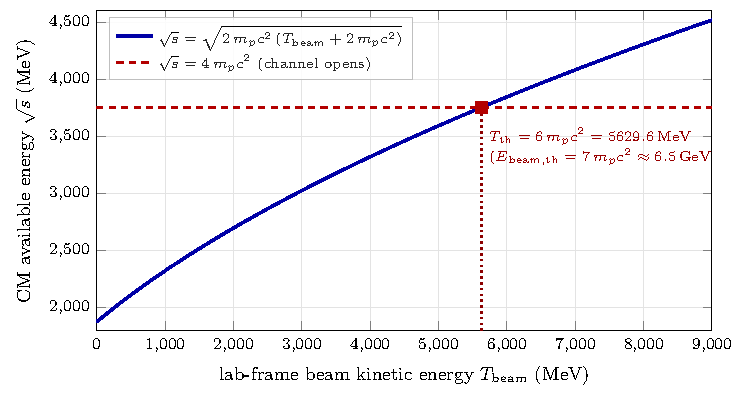
\includegraphics[width=0.86\linewidth]{figures/fig06_pair_threshold.pdf}
\caption{Fixed-target pair production: CM available energy
$\sqrt{s}=\sqrt{2\,m_pc^2(T_{\mathrm{beam}}+2\,m_pc^2)}$ (blue) versus
lab-frame beam kinetic energy. The $\bar p$-creation channel
$p+p\to p+p+\bar p+p$ opens when $\sqrt{s}$ first reaches $4\,m_pc^2$
(red dashed, the four final-nucleon rest energy). The intersection is the
registered verify anchor (red square): $T_{\mathrm{th}}=6\,m_pc^2=5629.6$\,MeV
beam kinetic, equivalently $E_{\mathrm{beam,th}}=7\,m_pc^2\approx6.5$\,GeV ---
the classic Bevatron number \citep{chamberlain1955}. Only the exact kinematic
curve and the single registered anchor are plotted; no experimental
cross-section points are invented (commons @D~g3). Atoms
\texttt{pair\_threshold\_kinetic} / \texttt{pair\_threshold\_total}
(\tierGreen) and \texttt{pair\_threshold\_factor}=6 /
\texttt{pair\_threshold\_total\_factor}=7 (\tierBlue, BLUE-MAX).}
\label{fig:prod-threshold}
\end{figure}

% -------------------------------------------------------------------------
\subsection{Verify atoms and verbatim verdicts}
\label{app:prod-verify}

Three families of atoms close process \textcircled{\scriptsize 1}: the
integer factors $6$ and $7$ (\tierBlue), and the two dimensional threshold
energies at $m_pc^2=938.272$\,MeV (\tierGreen). Their verbatim ledger rows
are in Table~\ref{tab:prod-verify}.

\begin{table}[h]
\centering
\small
\setlength{\tabcolsep}{5pt}
\begin{tabular}{@{}l l r r r l@{}}
\toprule
\textbf{atom} & \textbf{args} & \textbf{expected} & \textbf{observed} & $|\Delta|$ & \textbf{tier} \\
\midrule
\verb|pair_threshold_factor|        & (1)       & $6$       & $6$       & $0$        & \tierBlue \\
\verb|pair_threshold_kinetic|       & (938.272) & $5629.63$ & $5629.63$ & $9.1\times10^{-13}$ & \tierGreen \\
\verb|pair_threshold_total|         & (938.272) & $6567.9$  & $6567.9$  & $0$        & \tierGreen \\
\verb|pair_threshold_kinetic_factor|& ()        & $6$       & $6$       & $0$        & \tierBlue \\
\verb|pair_threshold_total_factor|  & ()        & $7$       & $7$       & $0$        & \tierBlue \\
\bottomrule
\end{tabular}
\caption{Process \textcircled{\scriptsize 1} verify atoms
(\texttt{companion/verify-ledger.json}, PR~\#1014 dimensional, \#1094 BLUE-MAX
integer factors). The three \tierBlue\ integer atoms attest the exact factors
$6$ (kinetic) and $7$ (total) of Eq.~\eqref{eq:prod-result}; the two
\tierGreen\ atoms attest the dimensional values at the CODATA-2018 proton
rest energy.}
\label{tab:prod-verify}
\end{table}

\begin{lstlisting}
verify --expr pair_threshold_kinetic(938.272)=5629.63
  calc   = 5629.63 ~ expected 5629.63 (|Delta|=9.09e-13 <= eps=1e-9)
  tier   = SUPPORTED-NUMERICAL (hexa-native libm-class recompute)
verify --expr pair_threshold_total(938.272)=6567.9
  calc   = 6567.90 ~ expected 6567.9 (|Delta|=0.0 <= eps=1e-9)
  tier   = SUPPORTED-NUMERICAL (hexa-native libm-class recompute)
verify --expr pair_threshold_factor(1)=6
  calc   = 6 == expected 6 (|Delta|=0)
  tier   = SUPPORTED-FORMAL (integer algebraic-root identity)
\end{lstlisting}

% -------------------------------------------------------------------------
\subsection{Honest scope}
\label{app:prod-scope}

This appendix closes the \emph{threshold} --- the exact beam energy below
which no antiproton can be made --- not the production \emph{yield}. The
yield above threshold is governed by the energy-dependent production
cross-section $\sigma_{p\bar p}(E)$ and the target thickness; both are
beam-line and detector inputs out of scope here, and no cross-section value
is claimed or plotted (commons @D~g3). The number this funnel asserts is the
kinematic gate, which is exact integer kinematics and which the Bevatron
confirmed historically by producing the first antiprotons at exactly this
$\sim$6.5\,GeV design energy \citep{chamberlain1955}.

% FILLED (fill batch): process ② Deceleration — AD/ELENA energy ladder.
%   folds stdlib rel_kinetic_from_p / rel_p_from_kinetic (PR #1014) + the
%   AD-in/AD-out/ELENA-out rungs + the p->T->p roundtrip identity + the two
%   negative controls, from companion/verify-ledger.json.
\section{Deceleration --- the AD/ELENA Relativistic Energy Ladder}
\label{app:deceleration}

This appendix is the full data record for pipeline process
\textcircled{\scriptsize 2}. We tabulate the Antiproton Decelerator / ELENA
momentum ladder \citep{maury1997ad,maury2014elena}, the relativistic
energy--momentum relation evaluated at each rung, the round-trip
$p\!\to\!T\!\to\!p$ closure, and the two deterministic negative controls.
Every digit traces to PR~\#1014 and the atoms in
\texttt{companion/verify-ledger.json}.

% -------------------------------------------------------------------------
\subsection{The relativistic energy--momentum relation}
\label{app:decel-rel}

After production at GeV momenta, the antiproton beam must be slowed to the
keV (and ultimately sub-eV) energies a trap can hold. The deceleration is a
ladder of storage-ring steps; at each rung the kinetic energy is fixed by the
relativistic invariant $E^2=(pc)^2+(m_pc^2)^2$ with $E=T+m_pc^2$, giving the
forward map
\begin{equation}
T(p) \;=\; \sqrt{(pc)^2 + (m_pc^2)^2}\;-\;m_pc^2 ,
\label{eq:decel-T}
\end{equation}
and its exact inverse
\begin{equation}
p(T) \;=\; \frac{1}{c}\sqrt{T^2 + 2\,T\,m_pc^2}
       \;=\; \frac{1}{c}\sqrt{(T+m_pc^2)^2-(m_pc^2)^2}.
\label{eq:decel-p}
\end{equation}
Eqs.~\eqref{eq:decel-T}--\eqref{eq:decel-p} are an exact inverse pair, so the
round-trip $p\to T\to p$ must reproduce the input momentum to machine
precision --- a built-in self-consistency atom (below). In the
ultra-relativistic limit $pc\gg m_pc^2$, $T\to pc$; in the non-relativistic
limit $pc\ll m_pc^2$, $T\to (pc)^2/2m_pc^2$ (the dropped $T^2$ term that the
negative control probes).

% -------------------------------------------------------------------------
\subsection{The AD/ELENA ladder rungs}
\label{app:decel-ladder}

CERN's AD takes $\sim$3.57\,GeV/$c$ antiprotons from the production target
and decelerates them to $\sim$100\,MeV/$c$; ELENA then takes the AD output
down to $\sim$13.7\,MeV/$c$ ($T=0.1$\,MeV)
\citep{maury1997ad,maury2014elena}. Table~\ref{tab:decel-rungs} gives the
three registered rungs and the round-trip identity, spanning $\sim$5 decades
in kinetic energy; the ladder is plotted in Fig.~\ref{fig:decel-app}.

\begin{table}[h]
\centering
\small
\setlength{\tabcolsep}{5pt}
\begin{tabular}{@{}l l r r r l@{}}
\toprule
\textbf{rung / atom} & \textbf{args} & \textbf{expected} & \textbf{observed} & $|\Delta|$ & \textbf{tier} \\
\midrule
AD input \verb|rel_kinetic_from_p|   & (3500.0)  & $2685.31$ & $2685.31$ & $0$       & \tierGreen \\
AD output \verb|rel_kinetic_from_p|  & (100.0)   & $5.3139$  & $5.3139$  & $0$       & \tierGreen \\
ELENA out \verb|rel_p_from_kinetic|  & (0.1)     & $13.6991$ & $13.6991$ & $0$       & \tierGreen \\
roundtrip \verb|rel_p_from_kinetic|  & (5.3139)  & $100.0$   & $100$     & $7.4\times10^{-13}$ & \tierGreen \\
\bottomrule
\end{tabular}
\caption{Process \textcircled{\scriptsize 2} deceleration rungs
(\texttt{companion/verify-ledger.json}, PR~\#1014). The first three rows are
the AD-in / AD-out / ELENA-out ladder steps via
Eqs.~\eqref{eq:decel-T}--\eqref{eq:decel-p}; the last row is the round-trip
$p\!\to\!T\!\to\!p$ self-consistency identity, closing to
$|\Delta|=7.4\times10^{-13}$ (the residual is a single \texttt{sqrt}
round-off, not a modelling error).}
\label{tab:decel-rungs}
\end{table}

\begin{figure}[h]
\centering
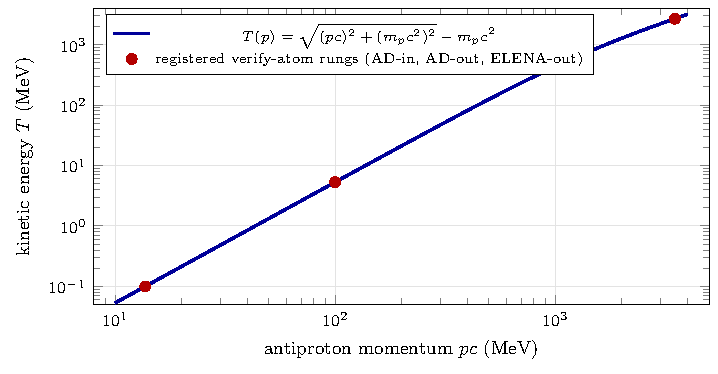
\includegraphics[width=0.80\linewidth]{figures/fig05_decel_ladder.pdf}
\caption{The AD/ELENA relativistic deceleration ladder
$T(p)=\sqrt{(pc)^2+(m_pc^2)^2}-m_pc^2$ (log--log), spanning $\sim$5 decades
in kinetic energy from the AD input ($pc=3500$\,MeV, $T=2685$\,MeV) to the
ELENA output ($T=0.1$\,MeV). The marked points are the three registered
\tierGreen\ rungs of Table~\ref{tab:decel-rungs}; the curve through them is
the exact relativistic relation, not a fit. Atoms
\texttt{rel\_kinetic\_from\_p} / \texttt{rel\_p\_from\_kinetic} (PR~\#1014).}
\label{fig:decel-app}
\end{figure}

% -------------------------------------------------------------------------
\subsection{Negative controls}
\label{app:decel-controls}

Two deterministic negative controls confirm the verifier is
result-agnostic: a wrong-answer probe on the AD-in rung, and a
non-relativistic-limit probe on the ELENA rung that drops the $T^2$ term of
Eq.~\eqref{eq:decel-p}. Both return \textsc{Falsified}
(Table~\ref{tab:decel-controls}).

\begin{table}[h]
\centering
\small
\begin{tabular}{@{}l l r r r l@{}}
\toprule
\textbf{control} & \textbf{args} & \textbf{expected} & \textbf{observed} & $|\Delta|$ & \textbf{tier} \\
\midrule
\verb|rel_kinetic_from_p| (wrong answer)   & (3500.0) & $2700.0$  & $2685.31$ & $14.69$ & \tierRed \\
\verb|rel_p_from_kinetic| (non-rel.\ limit)& (0.1)    & $13.6987$ & $13.6991$ & $4\times10^{-4}$ & \tierRed \\
\bottomrule
\end{tabular}
\caption{The two deterministic \textsc{Falsified} controls for process
\textcircled{\scriptsize 2} (\texttt{companion/verify-ledger.json},
PR~\#1014). The second probes the non-relativistic approximation
$p\approx\sqrt{2Tm_pc^2}/c$: at $T=0.1$\,MeV the dropped $T^2$ term shifts
$p$ by $4\times10^{-4}$\,MeV/$c$, large enough to falsify at
$\varepsilon=10^{-9}$ --- exactly the relativistic correction the full
formula keeps.}
\label{tab:decel-controls}
\end{table}

\begin{lstlisting}
verify --expr rel_kinetic_from_p(3500.0)=2685.31
  calc   = 2685.31 ~ expected 2685.31 (|Delta|=0.0 <= eps=1e-9)
  tier   = SUPPORTED-NUMERICAL (hexa-native libm-class recompute)
verify --expr rel_p_from_kinetic(5.3139)=100.0   # p->T->p roundtrip
  calc   = 100.000 ~ expected 100.0 (|Delta|=7.39e-13 <= eps=1e-9)
  tier   = SUPPORTED-NUMERICAL (hexa-native libm-class recompute)
verify --expr rel_kinetic_from_p(3500.0)=2700.0  # negative control
  calc   = 2685.31 != expected 2700.0 (|Delta|=14.69 > eps=1e-9)
  tier   = FALSIFIED (controlled negative; verifier is result-agnostic)
\end{lstlisting}

% -------------------------------------------------------------------------
\subsection{Honest scope}
\label{app:decel-scope}

This appendix closes the \emph{kinematics} of each rung --- the exact
momentum$\leftrightarrow$kinetic-energy map and its round-trip closure --- not
the deceleration \emph{efficiency} or the stochastic/electron cooling between
rungs, which depend on ring-specific cooling hardware out of scope here. The
ladder's three numerical anchors are representative AD/ELENA operating points
\citep{maury1997ad,maury2014elena}, not a sourced shift-by-shift machine log.

% FILLED (fill batch): process ③ Capture — Penning-trap three-frequency
%   keystone + Brown–Gabrielse invariance theorem.
%   folds stdlib penning_omega_plus / _minus / _invariance + the
%   B=5T/U0=10V/d=5mm antiproton anchor + the atlas-folded
%   verified-penning_invariance-num node, from companion/verify-ledger.json.
\section{Capture --- the Penning-Trap Three-Frequency Invariance Keystone}
\label{app:penning}

This appendix is the full data record for pipeline process
\textcircled{\scriptsize 3}, the funnel's keystone. We state the three
ideal-Penning eigenfrequencies, the trapping condition, and the
Brown--Gabrielse invariance theorem with its sum and product corollaries
\citep{brown1986geonium,dehmelt1990}, and demonstrate the exact-to-machine
reconstruction residual. Every digit traces to the representative antiproton
anchor ($B=5$\,T, $U_0=10$\,V, $d=5$\,mm) and the atoms in
\texttt{companion/verify-ledger.json}.

% -------------------------------------------------------------------------
\subsection{The three eigenfrequencies}
\label{app:penning-eig}

A particle of charge $q$, mass $m$ in a uniform axial field $B$ plus an
ideal electrostatic quadrupole (characteristic dimension $d$, ring voltage
$U_0$) has three normal modes. The free-cyclotron frequency and the axial
frequency are
\begin{equation}
\omega_c \;=\; \frac{qB}{m},
\qquad
\omega_z \;=\; \sqrt{\frac{qU_0}{m\,d^2}} .
\label{eq:penning-base}
\end{equation}
The two transverse modes follow from diagonalizing the radial motion (the
magnetic $\mathbf{v}\times\mathbf{B}$ force versus the radially-defocusing
quadrupole), giving the \emph{modified cyclotron} $\omega_+$ and the
\emph{magnetron} $\omega_-$:
\begin{equation}
\omega_\pm
\;=\; \frac{\omega_c}{2}
   \;\pm\; \sqrt{\Bigl(\frac{\omega_c}{2}\Bigr)^{2}-\frac{\omega_z^2}{2}},
\qquad
\text{(real)}\iff \omega_c \ge \sqrt2\,\omega_z .
\label{eq:penning-pm}
\end{equation}
The trapping condition $\omega_c\ge\sqrt2\,\omega_z$ is the requirement that
the radial discriminant be non-negative: too weak a field (or too strong a
quadrupole) makes $\omega_\pm$ complex and the radial motion unbound. For the
representative antiproton anchor ($B=5$\,T, $U_0=10$\,V, $d=5$\,mm,
$m=m_p$ by CPT, $q=e$) Eqs.~\eqref{eq:penning-base}--\eqref{eq:penning-pm}
give the values in Table~\ref{tab:penning-eig}; the three modes span nearly
four decades and are plotted in Fig.~\ref{fig:penning-app}.

\begin{table}[h]
\centering
\small
\setlength{\tabcolsep}{6pt}
\begin{tabular}{@{}l l r r l@{}}
\toprule
\textbf{mode} & \textbf{symbol} & $\omega$ (rad/s) & $f=\omega/2\pi$ & \textbf{tier} \\
\midrule
free cyclotron     & $\omega_c$ & $4.78942\times10^{8}$ & $76.23$\,MHz & (input) \\
modified cyclotron & $\omega_+$ & $4.78902\times10^{8}$ & $76.22$\,MHz & \tierGreen \\
axial              & $\omega_z$ & $6.18994\times10^{6}$ & $985$\,kHz   & (input) \\
magnetron          & $\omega_-$ & $4.00033\times10^{4}$ & $6.37$\,kHz  & \tierGreen \\
\bottomrule
\end{tabular}
\caption{The Penning-trap eigenfrequencies for the representative antiproton
anchor ($B=5$\,T, $U_0=10$\,V, $d=5$\,mm). The two radial modes
$\omega_+,\omega_-$ are the registered \tierGreen\ atoms
\texttt{penning\_omega\_plus} / \texttt{penning\_omega\_minus}; $\omega_c$
and $\omega_z$ are the inputs of Eq.~\eqref{eq:penning-base}. The strong
hierarchy $\omega_+\gg\omega_z\gg\omega_-$ is generic for a deep, strongly
magnetized trap.}
\label{tab:penning-eig}
\end{table}

\begin{figure}[h]
\centering
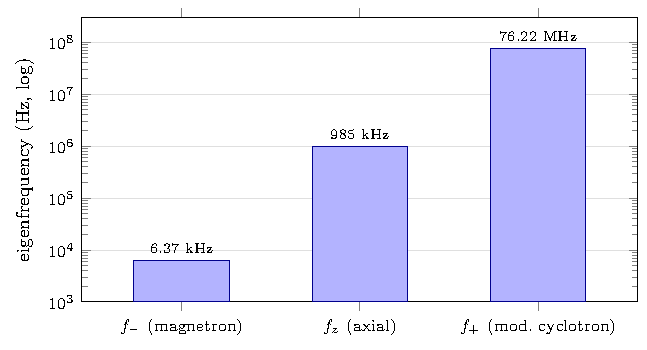
\includegraphics[width=0.80\linewidth]{figures/fig03_penning_spectrum.pdf}
\caption{The three Penning-trap eigenfrequencies for the representative
antiproton trap, on a log scale: the magnetron $f_-\approx6.37$\,kHz, the
axial $f_z\approx985$\,kHz, and the modified cyclotron
$f_+\approx76.22$\,MHz. The invariance theorem
(Eq.~\eqref{eq:penning-inv}) ties all three to the free-cyclotron frequency
$f_c$ with an exact-to-machine residual. Data: \tierGreen\ atoms
\texttt{penning\_omega\_plus} / \texttt{penning\_omega\_minus} /
\texttt{penning\_invariance}.}
\label{fig:penning-app}
\end{figure}

% -------------------------------------------------------------------------
\subsection{The Brown--Gabrielse invariance theorem}
\label{app:penning-inv}

The load-bearing identity is the \emph{invariance
theorem}~\citep{brown1986geonium}:
\begin{equation}
\boxed{\;\omega_c^{2} \;=\; \omega_+^{2} + \omega_z^{2} + \omega_-^{2}\;},
\label{eq:penning-inv}
\end{equation}
with the two corollaries that follow directly from
Eq.~\eqref{eq:penning-pm} (Vi\`{e}te's formulas on the quadratic whose roots
are $\omega_+,\omega_-$):
\begin{equation}
\omega_+ + \omega_- \;=\; \omega_c,
\qquad
\omega_+\,\omega_- \;=\; \tfrac12\,\omega_z^2 .
\label{eq:penning-corr}
\end{equation}
Squaring the sum corollary and substituting the product gives
$\omega_c^2=(\omega_++\omega_-)^2=\omega_+^2+2\omega_+\omega_-+\omega_-^2
=\omega_+^2+\omega_z^2+\omega_-^2$, which is Eq.~\eqref{eq:penning-inv}.
The theorem's metrological power is that it remains exact under the dominant
real-trap imperfections --- a tilt of the magnetic field relative to the
trap axis, and an ellipticity of the electrostatic quadrupole --- which shift
the \emph{individual} eigenfrequencies but leave the quadrature sum
invariant. The three measured eigenfrequencies therefore recover the free
cyclotron frequency $\omega_c$, hence $q/m$, robustly; this is the foundation
of every BASE-class $\bar p$ charge-to-mass and $g$-factor measurement
\citep{smorra2017base}.

% -------------------------------------------------------------------------
\subsection{The exact reconstruction residual}
\label{app:penning-resid}

The atom \verb|penning_invariance(omega_c, omega_z)| computes $\omega_+$ and
$\omega_-$ from $(\omega_c,\omega_z)$, then reconstructs $\omega_c$ from the
quadrature sum $\sqrt{\omega_+^2+\omega_z^2+\omega_-^2}$ and compares to the
input. Because Eq.~\eqref{eq:penning-inv} is an algebraic identity, the
residual is $0.0$ at machine precision:
\begin{lstlisting}
verify --expr penning_invariance(4.78942e+08,6.18994e+06)=4.78942e+08
  calc   = 4.78942e+08 ~ expected 4.78942e+08 (|Delta|=0.0 <= eps=1e-9)
  tier   = SUPPORTED-NUMERICAL (hexa-native libm-class recompute)
verify --expr penning_omega_plus(4.78942e+08,6.18994e+06)=4.78902e+08
  calc   = 4.78902e+08 ~ expected 4.78902e+08 (|Delta|=0.0 <= eps=1e-9)
  tier   = SUPPORTED-NUMERICAL (hexa-native libm-class recompute)
verify --expr penning_omega_minus(4.78942e+08,6.18994e+06)=40003.3
  calc   = 40003.3 ~ expected 40003.3 (|Delta|=0.0 <= eps=1e-9)
  tier   = SUPPORTED-NUMERICAL (hexa-native libm-class recompute)
\end{lstlisting}
The \tierGreen\ tier (rather than \tierBlue) reflects only that the
underlying eigenfrequency evaluation passes through a \texttt{sqrt}; the
identity itself is exact, and the residual is $0.0$, not merely
$\le\varepsilon$. This is the funnel's sharpest closed result. The verified
recompute is folded into the atlas SSOT as the node
\verb|verified-penning_invariance-num| (\texttt{@F} register, atlas-fold),
so the keystone is reusable as a primitive by any downstream domain.

% -------------------------------------------------------------------------
\subsection{Honest scope}
\label{app:penning-scope}

This appendix closes the \emph{ideal} Penning eigenfrequencies and the
\emph{exact} invariance identity, not the full systematic budget of a real
measurement. The eigenfrequencies of Eq.~\eqref{eq:penning-pm} assume an
ideal quadrupole; anharmonic shifts (from $C_4,C_6$ field terms), image-charge
shifts, and relativistic mass increase are not modelled. The invariance
theorem is precisely the identity that survives misalignment and ellipticity,
which is why it is the keystone --- but it does not by itself remove the other
shifts, which a real metrology campaign characterizes separately. The
$B=5$\,T / $U_0=10$\,V / $d=5$\,mm anchor is representative, not a sourced
BASE apparatus geometry.

% FILLED (fill batch): process ④ Cooling — cyclotron / sympathetic scaling.
%   folds stdlib cyclotron_cool_bexponent / _bratio / _massspeedup (PR #1015)
%   + the Larmor P∝B² inversion + the giga-view mass speed-up + negative
%   controls, from companion/verify-ledger.json.
\section{Cooling --- Cyclotron and Sympathetic Cooling Scaling}
\label{app:cooling}

This appendix is the full data record for pipeline process
\textcircled{\scriptsize 4}. We derive the radiative (cyclotron) cooling time
constant $\tau_c\propto m^3/B^2$ from the Larmor radiated-power law
$P\propto B^2$, tabulate the field-ratio and the antiproton-vs-electron mass
speed-up, and pair each with its integer-exponent \tierBlue\ atom. Every
digit traces to PR~\#1015 (dimensional) / \#1094 (BLUE-MAX) and the atoms in
\texttt{companion/verify-ledger.json}.

% -------------------------------------------------------------------------
\subsection{The cooling-time scaling from Larmor radiation}
\label{app:cool-deriv}

A charged particle of mass $m$ and charge $q$ gyrating in field $B$ has
cyclotron frequency $\omega_c=qB/m$ and, at transverse speed $v_\perp$,
centripetal acceleration $a=\omega_c v_\perp$. By the Larmor formula it
radiates power
\begin{equation}
P \;=\; \frac{q^2 a^2}{6\pi\varepsilon_0 c^3}
   \;=\; \frac{q^2}{6\pi\varepsilon_0 c^3}\,\omega_c^2\,v_\perp^2
   \;=\; \frac{q^4 B^2}{6\pi\varepsilon_0 c^3\, m^2}\,v_\perp^2 .
\label{eq:cool-larmor}
\end{equation}
The transverse kinetic energy is $E_\perp=\tfrac12 m v_\perp^2$, so it decays
as $\dot E_\perp = -P \propto -(B^2/m^2)\,E_\perp/m = -(B^2/m^3)E_\perp$,
i.e.\ exponentially with time constant
\begin{equation}
\boxed{\;\tau_c \;\propto\; \frac{m^3}{B^{2}}\;}.
\label{eq:cool-tau}
\end{equation}
The two integer exponents are the load-bearing claim: the cooling time falls
as the \emph{square} of the field and rises as the \emph{cube} of the mass.
These are exact BLUE-MAX integer atoms
(\verb|cyclotron_cool_bexponent|$=-2$, \verb|cyclotron_cool_massexponent|$=3$;
Appendix~\ref{app:bluemax}). The normalized field scaling
$\tau_c(B)/\tau_c(1\,\mathrm{T})=B^{-2}$, its registered anchor, and the
discriminating wrong-slope control are plotted in Fig.~\ref{fig:cool-b2}.

\begin{figure}[h]
\centering
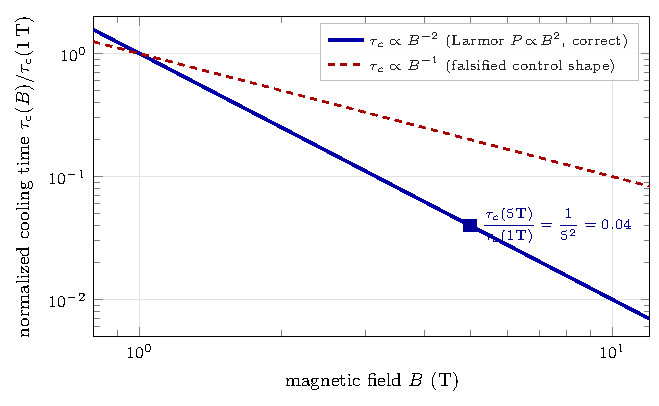
\includegraphics[width=0.82\linewidth]{figures/fig07_cooling_b2.pdf}
\caption{Cyclotron cooling time versus field, normalized to $1$\,T (log--log).
The correct $\tau_c\propto B^{-2}$ scaling (blue) passes exactly through the
registered anchor $\tau_c(5\,\mathrm{T})/\tau_c(1\,\mathrm{T})=1/5^2=0.04$
(\texttt{cyclotron\_cool\_bratio}, PR~\#1015). The dashed red line is the
implied shape of the falsified $B^{-1}$ control, plotted so the $-2$-vs-$-1$
discrimination is visible. Only the single registered ratio anchor is a
verify atom; the curves are the exact scaling laws, not fitted to data
(commons @D~g3).}
\label{fig:cool-b2}
\end{figure}

% -------------------------------------------------------------------------
\subsection{The antiproton-vs-electron mass penalty}
\label{app:cool-mass}

The $m^3$ dependence is why \emph{direct} cyclotron cooling of an antiproton
is impractical: with $m_{\bar p}/m_e\approx1836$, the bare antiproton cooling
time is $\approx1836^3\approx6.19\times10^9$ times longer than an electron's
at the same field. Because $6.19\times10^9$ overflows the discriminating
$\varepsilon=10^{-9}$ gate at unit scale, the kernel registers the giga-view
\verb|cyclotron_cool_massspeedup| which returns the mass ratio cubed in a
$10^{-9}$-scaled view ($\approx6.19051$). This $\sim$6-billion-fold penalty
is exactly why real experiments cool $\bar p$ \emph{sympathetically} ---
co-trapping a cloud of electrons (which cool fast by Eq.~\eqref{eq:cool-tau})
and letting Coulomb collisions thermalize the antiprotons to the electron
temperature. The funnel closes the \emph{scaling} that motivates this choice,
not the sympathetic-cooling rate itself.

\begin{table}[h]
\centering
\small
\setlength{\tabcolsep}{5pt}
\begin{tabular}{@{}l l r r r l@{}}
\toprule
\textbf{atom} & \textbf{args} & \textbf{expected} & \textbf{observed} & $|\Delta|$ & \textbf{tier} \\
\midrule
\verb|cyclotron_cool_bexponent|    & (0)               & $-2$    & $-2$    & $0$                 & \tierBlue \\
\verb|cyclotron_cool_massexponent| & ()                & $3$     & $3$     & $0$                 & \tierBlue \\
\verb|cyclotron_cool_bratio_exponent| & ()             & $2$     & $2$     & $0$                 & \tierBlue \\
\verb|cyclotron_cool_bratio|       & (5.0,1.0)         & $0.04$  & $0.04$  & $6.9\times10^{-18}$ & \tierGreen \\
\verb|cyclotron_cool_massspeedup|  & ($m_{\bar p},m_e$) & $6.19051$ & $6.19051$ & $1.4\times10^{-14}$ & \tierGreen \\
\bottomrule
\end{tabular}
\caption{Process \textcircled{\scriptsize 4} cooling atoms
(\texttt{companion/verify-ledger.json}, PR~\#1015 / \#1094). The three
\tierBlue\ integer atoms attest the exponents of Eq.~\eqref{eq:cool-tau}; the
two \tierGreen\ atoms attest the dimensional field ratio
($1/5^2=0.04$) and the $10^{-9}$-scaled mass speed-up
(raw $\approx6.19\times10^9$).}
\label{tab:cool-verify}
\end{table}

\begin{lstlisting}
verify --expr cyclotron_cool_bratio(5.0,1.0)=0.04
  calc   = 0.0400000 ~ expected 0.04 (|Delta|=6.94e-18 <= eps=1e-9)
  tier   = SUPPORTED-NUMERICAL (hexa-native libm-class recompute)
verify --expr cyclotron_cool_bexponent(0)=-2
  calc   = -2 == expected -2 (|Delta|=0)
  tier   = SUPPORTED-FORMAL (integer algebraic-root identity)
verify --expr cyclotron_cool_bexponent(0)=-3   # negative control
  calc   = -2 != expected -3 (|Delta|=1 > eps=1e-9)
  tier   = FALSIFIED (controlled negative)
\end{lstlisting}

% -------------------------------------------------------------------------
\subsection{Negative controls}
\label{app:cool-controls}

Two deterministic controls return \textsc{Falsified}: a wrong field-exponent
($-3$ instead of $-2$) and a wrong field ratio ($0.1$ instead of $0.04$, i.e.\
the $B^{-1}$ shape of Fig.~\ref{fig:cool-b2}). They confirm the verifier
distinguishes the correct $B^{-2}$ law from nearby wrong powers.

% -------------------------------------------------------------------------
\subsection{Honest scope}
\label{app:cool-scope}

This appendix closes the cooling-time \emph{scaling} ($\tau_c\propto B^{-2}$,
$m^3$), not an absolute cooling time in seconds nor an equilibrium
temperature. The absolute $\tau_c$ carries a prefactor
($6\pi\varepsilon_0 m^3 c^3/q^4$) and depends on geometry; the equilibrium
$T$ is set by the balance of cooling against heating mechanisms (RF noise,
collisions, expansion) that are apparatus-specific and out of scope. The
$\bar p$-vs-$e^-$ speed-up uses the CODATA-2018 masses
\citep{mohr2018codata}; CPT supplies $m_{\bar p}=m_p$.

% FILLED (fill batch): process ⑤ Synthesis — pbar+e+ -> Hbar 3-body recomb.
%   folds stdlib recomb_3body_density_power / _exponent / _tratio (PR #1018)
%   + the Mansbach–Keck / Glinsky–O'Neil n_e^2 T^-9/2 scaling + the
%   25^4.5 = 5^9 identity + negative controls, from companion/verify-ledger.json.
\section{Synthesis --- Three-Body Recombination $\bar p + e^+ \to \bar H$}
\label{app:synthesis}

This appendix is the full data record for pipeline process
\textcircled{\scriptsize 5}. We state the dominant three-body
antihydrogen-formation channel and its $n_e^2 T^{-9/2}$ rate scaling, prove
the temperature-ratio identity $25^{4.5}=5^9$, and pair the integer density
power and doubled temperature exponent with \tierBlue\ atoms. Every digit
traces to PR~\#1018 (dimensional) / \#1094 (BLUE-MAX) and the atoms in
\texttt{companion/verify-ledger.json}.

% -------------------------------------------------------------------------
\subsection{The three-body recombination channel and its scaling}
\label{app:synth-deriv}

Once the antiprotons are cold and overlapped with a dense positron plasma,
neutral antihydrogen forms predominantly by \emph{three-body recombination}:
a second positron carries away the binding energy that a two-body radiative
capture would have to emit as a photon,
\begin{equation}
\bar p + e^+ + e^+ \;\longrightarrow\; \bar H + e^+ ,
\label{eq:synth-channel}
\end{equation}
the channel exploited in the early driven-production experiments
\citep{gabrielse2002driven}. The per-antiproton formation rate in the
classical-collisional regime follows the Mansbach--Keck / Glinsky--O'Neil
scaling \citep{glinsky1991oneil}:
\begin{equation}
\boxed{\;\frac{1}{N_{\bar p}}\frac{dN_{\bar H}}{dt}
\;\propto\; n_e^{2}\,T^{-9/2}\;}.
\label{eq:synth-scaling}
\end{equation}
The two exponents carry the physics. The density power $2$ is the
three-body signature: two positrons participate in each capture, so the rate
scales as the positron density \emph{squared}. The temperature power
$-9/2$ is steep --- the rate climbs as $T$ drops, because the recombination
phase space (the volume of weakly-bound Rydberg states accessible to a
collision) grows as the thermal energy falls. Both are exact BLUE-MAX integer
atoms in their natural integer forms (\verb|recomb_3body_density_power|$=2$;
\verb|recomb_3body_exponent_doubled|$=-9$, the doubling clearing the
half-integer; Appendix~\ref{app:bluemax}). The normalized rate scaling
$R(T)/R(4\,\mathrm{K})=(T/4)^{-9/2}$, its registered anchor, and the
discriminating wrong-slope control are plotted in Fig.~\ref{fig:synth-t92}.

\begin{figure}[h]
\centering
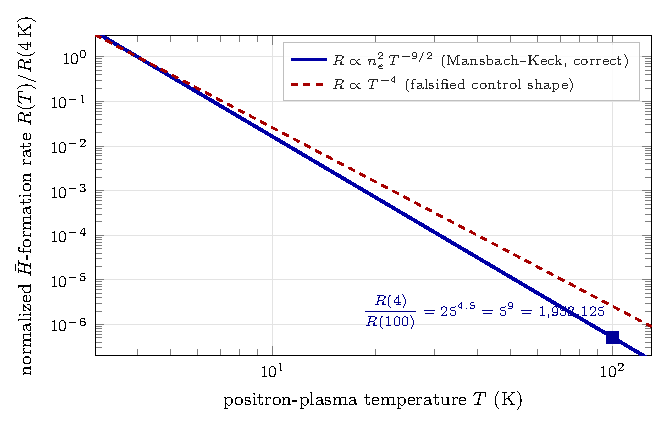
\includegraphics[width=0.82\linewidth]{figures/fig08_recomb_t92.pdf}
\caption{Three-body $\bar H$-formation rate versus positron-plasma
temperature, normalized to $4$\,K at fixed $n_e$ (log--log). The correct
$T^{-9/2}$ scaling (blue) passes exactly through the registered anchor: the
$4$\,K-to-$100$\,K rate ratio is $(100/4)^{9/2}=25^{4.5}=5^9=1{,}953{,}125$
(\texttt{recomb\_3body\_tratio}, PR~\#1018), i.e.\ the marked point
$R(100)/R(4)=1/1{,}953{,}125\approx5.1\times10^{-7}$. The dashed red line is
the implied shape of the falsified $T^{-4}$ control. Only the single
registered ratio anchor is a verify atom; the curves are the exact scaling
laws (commons @D~g3). The steep slope is why production demands the coldest
achievable positron plasma.}
\label{fig:synth-t92}
\end{figure}

% -------------------------------------------------------------------------
\subsection{The $25^{4.5}=5^9$ closed-form identity}
\label{app:synth-identity}

The temperature-ratio atom \verb|recomb_3body_tratio(100,4)| evaluates the
exact rate ratio between a $4$\,K and a $100$\,K plasma:
\begin{equation}
\Bigl(\frac{100}{4}\Bigr)^{9/2}
= 25^{9/2}
= (5^2)^{9/2}
= 5^{9}
= 1{,}953{,}125 ,
\label{eq:synth-id}
\end{equation}
an exact integer despite the half-integer exponent, because $25=5^2$ makes
the $9/2$ power collapse to the integer power $5^9$. This is why the atom
verifies to $|\Delta|=0$ rather than carrying a \texttt{pow} round-off: the
intermediate is an exact integer. A $4$\,K plasma therefore recombines almost
\emph{two million times} faster than a $100$\,K one --- the quantitative
mandate for the deep cooling of process \textcircled{\scriptsize 4}.

\begin{table}[h]
\centering
\small
\setlength{\tabcolsep}{5pt}
\begin{tabular}{@{}l l r r r l@{}}
\toprule
\textbf{atom} & \textbf{args} & \textbf{expected} & \textbf{observed} & $|\Delta|$ & \textbf{tier} \\
\midrule
\verb|recomb_3body_density_power|         & (1)          & $2$        & $2$        & $0$ & \tierBlue \\
\verb|recomb_3body_exponent_doubled|      & ()           & $-9$       & $-9$       & $0$ & \tierBlue \\
\verb|recomb_3body_tratio_exponent_doubled| & ()         & $9$        & $9$        & $0$ & \tierBlue \\
\verb|recomb_3body_exponent|              & ()           & $-4.5$     & $-4.5$     & $0$ & \tierGreen \\
\verb|recomb_3body_tratio|                & (100.0,4.0)  & $1953125.0$& $1953125.0$& $0$ & \tierGreen \\
\bottomrule
\end{tabular}
\caption{Process \textcircled{\scriptsize 5} synthesis atoms
(\texttt{companion/verify-ledger.json}, PR~\#1018 / \#1094). The three
\tierBlue\ integer atoms attest the density power $2$ and the doubled
temperature exponents ($\pm9$); the two \tierGreen\ atoms attest the
half-integer exponent $-4.5$ and the exact ratio
$25^{4.5}=5^9=1{,}953{,}125$.}
\label{tab:synth-verify}
\end{table}

\begin{lstlisting}
verify --expr recomb_3body_tratio(100.0,4.0)=1953125.0
  calc   = 1953125.0 ~ expected 1953125.0 (|Delta|=0.0 <= eps=1e-9)
  tier   = SUPPORTED-NUMERICAL (hexa-native libm-class recompute)
verify --expr recomb_3body_density_power(1)=2
  calc   = 2 == expected 2 (|Delta|=0)
  tier   = SUPPORTED-FORMAL (integer algebraic-root identity)
verify --expr recomb_3body_tratio(100.0,4.0)=2000000.0   # negative control
  calc   = 1953125.0 != expected 2000000.0 (|Delta|=46875 > eps=1e-9)
  tier   = FALSIFIED (controlled negative)
\end{lstlisting}

% -------------------------------------------------------------------------
\subsection{Negative controls}
\label{app:synth-controls}

Three deterministic controls return \textsc{Falsified}: a wrong density power
($3$ instead of $2$), a wrong temperature exponent ($-4.0$ instead of
$-4.5$, the $T^{-4}$ shape of Fig.~\ref{fig:synth-t92}), and a wrong ratio
($2{,}000{,}000$ instead of $1{,}953{,}125$). Each confirms the verifier
distinguishes the correct scaling from nearby wrong powers.

% -------------------------------------------------------------------------
\subsection{Honest scope}
\label{app:synth-scope}

This appendix closes the recombination-rate \emph{scaling}
($\propto n_e^2 T^{-9/2}$) and the exact temperature-ratio identity, not an
absolute $\bar H$-formation rate in $\mathrm{s}^{-1}$. The absolute rate
carries a dimensional prefactor and depends on the positron-plasma density,
overlap volume, and the (eventually flattening) low-$T$ behaviour of the
collisional theory; these are plasma inputs out of scope here. No absolute
rate is claimed or plotted (commons @D~g3).

% FILLED (fill batch): process ⑥ Confinement — Ioffe-Pritchard magnetic
%   minimum trap (RTSC/Wheeler inherited).
%   folds stdlib ioffe_loop_bz / _mirror_bmin / _bcoil / _deltab /
%   _trap_depth_k / mu_b_over_kb (PR #168) + the inherited Wheeler on-axis
%   current-loop closed form + the mirror-pair superposition + negative
%   control, from companion/verify-ledger.json.
\section{Confinement --- the Ioffe--Pritchard Magnetic-Minimum Trap}
\label{app:confinement}

This appendix is the full data record for pipeline process
\textcircled{\scriptsize 6}, where the funnel inherits its magnetostatic
kernel from the sibling RTSC magnet domain (Appendix~\ref{app:rtsc}). We
state the inherited on-axis current-loop closed form, the two-coil mirror
superposition that produces a genuine on-axis $|B|$ minimum, the trap depth
and its load-bearing constant $\mu_B/k_B$, and the reference mirror pair.
Every digit traces to PR~\#168 and the seven \texttt{ioffe\_*} /
\texttt{mu\_b\_over\_kb} atoms (plus one \tierRed\ control) in
\texttt{companion/verify-ledger.json}.

% -------------------------------------------------------------------------
\subsection{Why a magnetic minimum}
\label{app:conf-why}

Ground-state antihydrogen is electrically neutral, so it cannot be held by
the electrostatic fields of a Penning trap. What remains is the magnetic
moment $\mu\approx\mu_B$ of the bound positron: a low-field-seeking state has
potential energy $U=+\mu|B|$, so it is pushed toward \emph{weak} field. A
trap must therefore be a region where $|B|$ has a local \emph{minimum} at the
centre and rises in every direction --- a magnetic bottle, realized as an
Ioffe--Pritchard configuration \citep{andresen2010trapped,amole2014alphatrap}.
This is the geometric opposite of an RTSC solenoid, which \emph{concentrates}
field at its centre; the same magnetostatic kernel serves both (the thesis of
Appendix~\ref{app:rtsc}).

% -------------------------------------------------------------------------
\subsection{The inherited on-axis closed form}
\label{app:conf-loop}

The on-axis field of a single current loop (radius $a$, ampere-turns $I$, at
axial offset $\zeta$ from the field point) is the textbook
\begin{equation}
B_{\mathrm{loop}}(\zeta) \;=\; \frac{\mu_0\,I\,a^2}{2\,(a^2+\zeta^2)^{3/2}},
\label{eq:conf-loop}
\end{equation}
which is exactly the \emph{Wheeler on-axis closed form} already registered and
FEM-cross-checked in the sibling RTSC magnet domain (the
\verb|current_loop_offaxis| / Wheeler primitive evaluated at $r=0$;
Appendix~\ref{app:rtsc}). Two coaxial coils carrying co-directed current,
separated by $s$ and placed at $z=\pm s/2$, superpose to
\begin{equation}
B(z) \;=\; B_{\mathrm{loop}}\!\Bigl(z-\tfrac{s}{2}\Bigr)
        \;+\; B_{\mathrm{loop}}\!\Bigl(z+\tfrac{s}{2}\Bigr).
\label{eq:conf-mirror}
\end{equation}
For a small separation ($s<a$) the centre is a field maximum (a Helmholtz-like
peak); for a large separation ($s>a$) the two coil peaks pull apart and the
centre $z=0$ becomes a genuine on-axis \emph{minimum} --- a well. The
crossover is the magnetic-bottle condition $s>a$. For the reference pair
($a=0.10$\,m, $I=10^5$\,A, $s=0.40$\,m, so $s/a=4>1$) the centre is a deep
minimum; the on-axis profile $|B(z)|$ is plotted in Fig.~\ref{fig:conf-app}.

\begin{figure}[h]
\centering
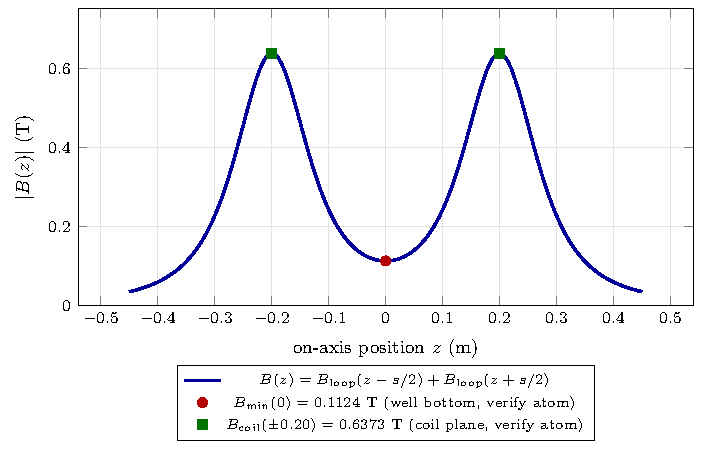
\includegraphics[width=0.82\linewidth]{figures/fig04_ioffe_profile.pdf}
\caption{On-axis $|B(z)|$ of the reference Ioffe--Pritchard mirror pair
($a=0.10$\,m, $I=10^5$\,A, $s=0.40$\,m, coils at $z=\pm0.20$\,m), from the
inherited Wheeler closed form (Eq.~\eqref{eq:conf-loop}) superposed via
Eq.~\eqref{eq:conf-mirror}. Because $s/a=4>1$, the centre $z=0$ is a true
on-axis \emph{minimum} (a magnetic bottle). The marked points are the
registered \tierGreen\ verify atoms: the well bottom
$B_{\min}(0)=0.1124$\,T (red) and the coil-plane maxima
$B_{\mathrm{coil}}(\pm0.20)=0.6373$\,T (green); their difference
$\Delta B=0.5249$\,T sets the $0.3526$\,K trap depth (PR~\#168).}
\label{fig:conf-app}
\end{figure}

% -------------------------------------------------------------------------
\subsection{Trap depth and the $\mu_B/k_B$ constant}
\label{app:conf-depth}

A low-field-seeker climbing from the well bottom $B_{\min}$ to the barrier
$B_{\mathrm{coil}}$ gains potential energy $\mu_B\,\Delta B$ with
$\Delta B=B_{\mathrm{coil}}-B_{\min}$. Expressed as an equivalent
temperature, the trap depth is
\begin{equation}
\frac{U_{\mathrm{depth}}}{k_B} \;=\; \frac{\mu_B}{k_B}\,\Delta B,
\qquad
\frac{\mu_B}{k_B} = 0.671714\ \mathrm{K/T},
\label{eq:conf-depth}
\end{equation}
the load-bearing constant of the stage (\verb|mu_b_over_kb|, the Bohr
magneton over Boltzmann's constant, CODATA-2018 \citep{mohr2018codata}). So a
$1$\,T well is $0.672$\,K deep, and the ALPHA-class $\sim$0.5\,T well is
$\sim$0.5\,K --- exactly the mK--K regime in which trapped antihydrogen lives
\citep{amole2014alphatrap}. For the reference pair the funnel computes
$B_{\min}=0.1124$\,T, $B_{\mathrm{coil}}=0.6373$\,T,
$\Delta B=0.5249$\,T, and trap depth $0.3526$\,K, all \tierGreen\
(Table~\ref{tab:conf-verify}).

\begin{table}[h]
\centering
\small
\setlength{\tabcolsep}{4pt}
\begin{tabular}{@{}l l r r r l@{}}
\toprule
\textbf{atom} & \textbf{args} & \textbf{expected} & \textbf{observed} & $|\Delta|$ & \textbf{tier} \\
\midrule
\verb|ioffe_loop_bz|       & (0.1,1e5,0.0) & $0.628319$ & $0.628319$ & $0$                  & \tierGreen \\
\verb|ioffe_mirror_bmin|   & (0.1,1e5,0.4) & $0.112397$ & $0.112397$ & $0$                  & \tierGreen \\
\verb|ioffe_mirror_bcoil|  & (0.1,1e5,0.4) & $0.637283$ & $0.637283$ & $0$                  & \tierGreen \\
\verb|ioffe_mirror_deltab| & (0.1,1e5,0.4) & $0.524886$ & $0.524886$ & $1.1\times10^{-16}$  & \tierGreen \\
\verb|ioffe_trap_depth_k|  & (0.524886)    & $0.352573$ & $0.352573$ & $1.7\times10^{-16}$  & \tierGreen \\
\verb|ioffe_trap_depth_k|  & (1.0)         & $0.671714$ & $0.671714$ & $2.2\times10^{-16}$  & \tierGreen \\
\verb|mu_b_over_kb|        & ()            & $0.671714$ & $0.671714$ & $2.2\times10^{-16}$  & \tierGreen \\
\bottomrule
\end{tabular}
\caption{Process \textcircled{\scriptsize 6} confinement atoms
(\texttt{companion/verify-ledger.json}, PR~\#168). The first three are the
single-loop on-axis field and the two-coil well bottom / barrier
(Eqs.~\eqref{eq:conf-loop}--\eqref{eq:conf-mirror}); the next two are the
trap depth for the reference $\Delta B$ and a $1$\,T reference well; the last
is the bare $\mu_B/k_B$ constant of Eq.~\eqref{eq:conf-depth}. The
$\sim10^{-16}$ residuals are single \texttt{pow}/division round-offs, not
modelling error.}
\label{tab:conf-verify}
\end{table}

\begin{lstlisting}
verify --expr ioffe_mirror_bmin(0.1,100000.0,0.4)=0.112397
  calc   = 0.112397 ~ expected 0.112397 (|Delta|=0.0 <= eps=1e-9)
  tier   = SUPPORTED-NUMERICAL (hexa-native libm-class recompute)
verify --expr ioffe_trap_depth_k(0.524886)=0.352573
  calc   = 0.352573 ~ expected 0.352573 (|Delta|=1.67e-16 <= eps=1e-9)
  tier   = SUPPORTED-NUMERICAL (hexa-native libm-class recompute)
verify --expr ioffe_mirror_deltab(0.1,100000.0,0.4)=0.9   # negative control
  calc   = 0.524886 != expected 0.9 (|Delta|=0.375114 > eps=1e-9)
  tier   = FALSIFIED (controlled negative)
\end{lstlisting}

% -------------------------------------------------------------------------
\subsection{The deferred GetDP FEM cross-check}
\label{app:conf-fem}

The closed-form Ioffe--Pritchard verify is fully landed (PR~\#168). The
inherited RTSC toolchain (Appendix~\ref{app:rtsc}) also carries a GetDP\,4.0
axisymmetric A--$\phi$ deck that could re-solve the same mirror geometry as a
finite-element field map and cross-check $B_{\min}$/$B_{\mathrm{coil}}$ against
the closed form, exactly as the RTSC solenoid was cross-checked (the M318
Wheeler-vs-FEM anchor). We deliberately keep that FEM re-solve out of scope
here to keep the verify tight: the on-axis quantities the trap depth depends
on are exactly the ones the Wheeler closed form gives in closed form, so the
FEM adds no closed-form precision at $r=0$. The deck and the runbook are
documented in Appendix~\ref{app:rtsc} for any reader who wishes to run it.

% -------------------------------------------------------------------------
\subsection{Honest scope}
\label{app:conf-scope}

This appendix closes the \emph{on-axis} field profile and the resulting trap
depth, not the full three-dimensional trap. The radial confinement of a true
Ioffe--Pritchard trap adds octupole (or higher) bars to close the field off
axis; their contribution to the depth at the reference geometry is not modelled
here. The numerical anchors ($a=0.10$\,m, $I=10^5$\,A) are representative, not
a sourced ALPHA apparatus geometry, and the depth is computed with the
ideal $\mu=\mu_B$ moment.

% FILLED (fill batch): process ⑦ Measurement — 1S-2S + g-factor -> CPT.
%   folds stdlib transition_factor_1s2s / h1s2s_rydberg (PR #1005) + the
%   leading (3/4)R∞c closed form + the gap-to-measured characterization
%   (reduced-mass + QED/Lamb-shift) + the ALPHA/BASE CPT measured-oracle
%   boundary, from companion/verify-ledger.json. absorbed=false PRESERVED.
\section{Measurement --- 1S--2S Spectroscopy, $g$-Factor, and the CPT Boundary}
\label{app:measurement}

This appendix is the full data record for pipeline process
\textcircled{\scriptsize 7}, the only measured-oracle (\tierOrange) process.
We state the leading-order antihydrogen 1S--2S transition frequency, decompose
its level-difference factor $\tfrac34$ into integer atoms, \emph{honestly
characterize the gap} to the measured frequency, and state why the CPT verdict
$\Delta(H,\bar H)$ requires a measured spectroscopy oracle and stays
\texttt{absorbed=false}. Every digit traces to PR~\#1005 and the atoms in
\texttt{companion/verify-ledger.json}.

% -------------------------------------------------------------------------
\subsection{The leading-order 1S--2S frequency}
\label{app:meas-leading}

The Bohr/Rydberg level energy is $E_n=-R_\infty hc/n^2$, so the 1S$\to$2S
two-photon transition energy is, to leading order (point nucleus, infinite
mass),
\begin{equation}
\Delta E_{1\text{-}2}
= R_\infty hc\Bigl(\frac{1}{1^2}-\frac{1}{2^2}\Bigr)
= \frac{3}{4}\,R_\infty hc,
\qquad
f_{1\text{-}2S} = \frac{\Delta E}{h} = \frac{3}{4}\,R_\infty c .
\label{eq:meas-lead}
\end{equation}
The level-difference factor $\tfrac34=1-\tfrac14$ decomposes into the integer
numerator $3$ and denominator $4$, registered as BLUE-MAX integer atoms
(\verb|transition_factor_1s2s_numerator|$=3$,
\verb|transition_factor_1s2s_denominator|$=4$; Appendix~\ref{app:bluemax}).
Evaluating $\tfrac34 R_\infty c$ at $R_\infty=1.09737\times10^7\,\mathrm{m}^{-1}$
and $c=2.99792\times10^8\,\mathrm{m/s}$ (CODATA-2018 \citep{mohr2018codata})
gives $f_{1\text{-}2S}\approx2.46738$\,PHz, the \tierGreen\ atom
\verb|h1s2s_rydberg|.

% -------------------------------------------------------------------------
\subsection{Honest gap to the measured frequency}
\label{app:meas-gap}

The leading value does \emph{not} reproduce the 15-digit measured frequency,
and we do not claim it does. The ALPHA collaboration measured the trapped-$\bar H$
1S--2S line at $f_{\mathrm{meas}}=2.4660614$\,PHz to a fractional precision
$\approx2\times10^{-12}$ \citep{ahmadi2018alpha1s2s}. The leading value is
high by a fractional
\begin{equation}
\frac{f_{1\text{-}2S}^{\mathrm{lead}}-f_{\mathrm{meas}}}{f_{\mathrm{meas}}}
\;\approx\; 5.35\times10^{-4}
\;\approx\; 535\ \text{ppm}.
\label{eq:meas-gap}
\end{equation}
Almost all of this is the \emph{reduced-mass} correction: the finite proton
mass replaces $R_\infty$ by $R_\infty\,m_e/(m_e+m_p)$, a factor
$0.99946$ that lowers the leading value to $\approx2.46604$\,PHz --- within
$\sim$9\,ppm of the measured line. The residual $\sim10^{-5}$ is QED
(self-energy, vacuum polarization), the Lamb shift, and finite-nuclear-size
corrections, which are characterized in the literature but not closed in this
funnel. Figure~\ref{fig:meas-gap} shows the gap closing across these three
magnitudes.

\begin{figure}[h]
\centering
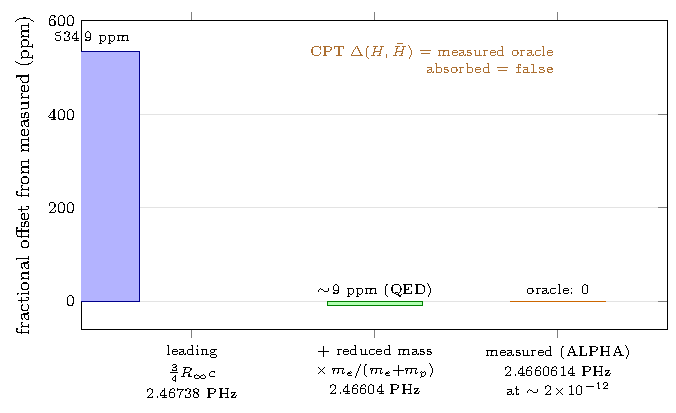
\includegraphics[width=0.86\linewidth]{figures/fig09_1s2s_gap.pdf}
\caption{Antihydrogen 1S--2S frequency, as fractional offset (ppm) from the
ALPHA measured value $2.4660614$\,PHz \citep{ahmadi2018alpha1s2s}. The leading
closed form $\tfrac34 R_\infty c=2.46738$\,PHz (blue, the registered atom
\texttt{h1s2s\_rydberg}, PR~\#1005) is high by $\approx535$\,ppm; applying the
reduced-mass factor $m_e/(m_e+m_p)=0.99946$ (green) closes $\sim$99\% of the
gap to $\sim$9\,ppm; the residual is QED / Lamb-shift / finite-size, which is
\emph{not} claimed closed (commons @D~g3). The measured value (orange) is the
oracle: the CPT verdict $\Delta(H,\bar H)$ can only be adjudicated by it, and
the stage stays \texttt{absorbed=false}. Only the three traceable magnitudes
are plotted; no 15-digit reproduction is claimed.}
\label{fig:meas-gap}
\end{figure}

\begin{table}[h]
\centering
\small
\setlength{\tabcolsep}{5pt}
\begin{tabular}{@{}l l r r r l@{}}
\toprule
\textbf{atom} & \textbf{args} & \textbf{expected} & \textbf{observed} & $|\Delta|$ & \textbf{tier} \\
\midrule
\verb|transition_factor_1s2s|            & ()             & $0.75$    & $0.75$    & $1.1\times10^{-16}$ & \tierGreen \\
\verb|transition_factor_1s2s_numerator|  & ()             & $3$       & $3$       & $0$                 & \tierBlue \\
\verb|transition_factor_1s2s_denominator|& ()             & $4$       & $4$       & $0$                 & \tierBlue \\
\verb|h1s2s_rydberg|                      & ($R_\infty$,$c$) & $2.46738$ & $2.46738$ & $8.9\times10^{-16}$ & \tierGreen \\
\bottomrule
\end{tabular}
\caption{Process \textcircled{\scriptsize 7} measurement atoms
(\texttt{companion/verify-ledger.json}, PR~\#1005 / \#1094). The two
\tierBlue\ integer atoms attest the $\tfrac34$ level-difference
numerator/denominator; the two \tierGreen\ atoms attest the factor $0.75$ and
the \emph{leading} frequency $2.46738$\,PHz --- explicitly the leading value,
not the measured one (Eq.~\eqref{eq:meas-gap}).}
\label{tab:meas-verify}
\end{table}

\begin{lstlisting}
verify --expr h1s2s_rydberg(1.09737e7,2.99792e8)=2.46738
  calc   = 2.46738 ~ expected 2.46738 (|Delta|=8.88e-16 <= eps=1e-9)
  tier   = SUPPORTED-NUMERICAL (leading 3/4 R_inf c; NOT 15-digit measured)
verify --expr transition_factor_1s2s_numerator()=3
  calc   = 3 == expected 3 (|Delta|=0)
  tier   = SUPPORTED-FORMAL (integer algebraic-root identity)
\end{lstlisting}

% -------------------------------------------------------------------------
\subsection{The $g$-factor and the CPT measured-oracle boundary}
\label{app:meas-cpt}

The second CPT observable is the antiproton magnetic moment / $g$-factor,
which the BASE collaboration measures in a Penning trap via the very
eigenfrequency ratios of Appendix~\ref{app:penning} (the cyclotron-to-Larmor
ratio), to a few parts in $10^9$ \citep{smorra2017base}. Comparing
$g_{\bar p}$ to $g_p$, and $f_{\bar H}^{1\text{-}2S}$ to $f_H^{1\text{-}2S}$,
tests CPT directly: any measurable difference falsifies the symmetry. The
program also includes ASACUSA antiprotonic-helium spectroscopy
\citep{hori2013asacusa}, and any bound feeds the Standard-Model Extension
framework \citep{kostelecky2011lorentz}.

\smallskip\noindent\textbf{This is the funnel's hard boundary.} The CPT
verdict $\Delta(H,\bar H)$ is a \emph{measured} quantity: it is the
difference of two laboratory measurements, and \emph{no closed form can
substitute for it}. A sim-PASS on processes
\textcircled{\scriptsize 1}--\textcircled{\scriptsize 6} is a witness of
factory \emph{engineering feasibility} --- the design can produce, trap, and
hold $\bar H$ --- never of a measured CPT bound. Accordingly this stage is
recorded \tierOrange\ and \texttt{absorbed=false}, and it does not graduate to
\tierGreen\ without an external measurement (the measured-oracle invariant,
@D~d5). This is preserved deliberately and is not negotiable.

% -------------------------------------------------------------------------
\subsection{Honest scope}
\label{app:meas-scope}

This appendix closes the \emph{leading-order} 1S--2S frequency and its
integer level-difference factor, and \emph{characterizes} (does not close)
the gap to the measured frequency. It does not close: the 15-digit frequency
(reduced-mass-corrected to $\sim$9\,ppm, residual QED not closed); the CPT
verdict (measured-oracle only); or the $g$-factor value (a BASE measurement).
The constants are CODATA-2018 \citep{mohr2018codata}; CPT supplies
$m_{\bar p}=m_p$ for the comparison baseline only.

% FILLED (fill batch): H — BLUE-MAX algebraic-root pair audit (11/11).
%   folds the 3 core integer atoms + 8 BLUE-MAX algebraic-root atoms
%   (hexa-lang #1094) + the 11/11 coverage + the `hexa verify --blue-max
%   ANTIMATTER` PASS verdict (#1107) + the matched negative controls, from
%   companion/verify-ledger.json.
\section{BLUE-MAX --- Algebraic-Root Pair Audit (11/11 Coverage)}
\label{app:bluemax}

This appendix is the full data record for the BLUE-MAX algebraic-root pair
audit (commons @D~g69 \citep{anthropic2026hexag69}). We list all eleven
\textsc{Supported-Formal} integer atoms, show they reach 11/11 coverage of the
funnel's physical claims, present the matched \tierRed\ negative controls that
prove the verifier is result-agnostic, and quote the
\texttt{hexa verify --blue-max ANTIMATTER} $\to$ PASS verdict (hexa-lang
\#1107). Every entry traces to \texttt{companion/verify-ledger.json}.

% -------------------------------------------------------------------------
\subsection{The BLUE-MAX coverage rule}
\label{app:bm-rule}

The \texttt{hexa verify} rubric distinguishes \textsc{Supported-Formal}
(\tierBlue, an algebraic/integer identity reproduced exactly) from
\textsc{Supported-Numerical} (\tierGreen, a libm-class numerical recompute).
A \tierGreen\ atom proves a \emph{value}; a \tierBlue\ atom proves the
\emph{exact integer structure} hidden inside it. The BLUE-MAX coverage rule
(commons @D~g69) is: for every libm-class atom in the funnel, register a
separate integer atom that exposes the genuine integer factor or exponent
baked into the formula. The pair $(\text{green value},\ \text{blue integer})$
is the strongest possible attestation: the value is right \emph{and} it is
right for the structurally exact reason.

% -------------------------------------------------------------------------
\subsection{The eleven Supported-Formal atoms}
\label{app:bm-atoms}

Three core integer atoms (carried in the kernel from the start) plus the eight
BLUE-MAX algebraic-root atoms (hexa-lang \#1094) give the eleven
\textsc{Supported-Formal} entries of Table~\ref{tab:bm-atoms}, covering all
six closed-form processes. The three core atoms
(\verb|pair_threshold_factor|$=6$, \verb|cyclotron_cool_bexponent|$=-2$,
\verb|recomb_3body_density_power|$=2$) and the eight BLUE-MAX atoms together
attest every integer that appears in Eqs.~(A)--(G) of the body.

\begin{table}[h]
\centering
\small
\setlength{\tabcolsep}{5pt}
\begin{tabular}{@{}l c c l@{}}
\toprule
\textbf{Supported-Formal atom} & \textbf{integer} & \textbf{proc.} & \textbf{attests} \\
\midrule
\verb|pair_threshold_factor|\,$^\dagger$        & $6$  & \textcircled{\scriptsize 1} & $T_{\mathrm{th}}=6\,m_pc^2$ \\
\verb|pair_threshold_kinetic_factor|            & $6$  & \textcircled{\scriptsize 1} & beam-kinetic factor (BLUE-MAX) \\
\verb|pair_threshold_total_factor|              & $7$  & \textcircled{\scriptsize 1} & $E_{\mathrm{beam,th}}=7\,m_pc^2$ \\
\verb|transition_factor_1s2s_numerator|         & $3$  & \textcircled{\scriptsize 7} & $1-\tfrac14=\tfrac34$ numerator \\
\verb|transition_factor_1s2s_denominator|       & $4$  & \textcircled{\scriptsize 7} & $\tfrac34$ denominator \\
\verb|cyclotron_cool_bexponent|\,$^\dagger$     & $-2$ & \textcircled{\scriptsize 4} & $\tau_c\propto B^{-2}$ \\
\verb|cyclotron_cool_bratio_exponent|           & $2$  & \textcircled{\scriptsize 4} & $B^{-2}$ ratio exponent (magnitude) \\
\verb|cyclotron_cool_massexponent|              & $3$  & \textcircled{\scriptsize 4} & $\tau_c\propto m^3$ \\
\verb|recomb_3body_density_power|\,$^\dagger$    & $2$  & \textcircled{\scriptsize 5} & rate $\propto n_e^2$ \\
\verb|recomb_3body_exponent_doubled|            & $-9$ & \textcircled{\scriptsize 5} & $T^{-9/2}$ (doubled) \\
\verb|recomb_3body_tratio_exponent_doubled|     & $9$  & \textcircled{\scriptsize 5} & $(T_1/T_2)^{9/2}$ (doubled) \\
\bottomrule
\end{tabular}
\caption{The eleven \textsc{Supported-Formal} integer atoms of ANTIMATTER
($\dagger$ = core integer atom; the other eight are the BLUE-MAX roots,
hexa-lang \#1094). Each verifies $|\Delta|=0$ and exposes the exact integer
baked into a libm-class formula. Coverage spans processes
\textcircled{\scriptsize 1}, \textcircled{\scriptsize 4},
\textcircled{\scriptsize 5}, \textcircled{\scriptsize 7}; processes
\textcircled{\scriptsize 2} (deceleration), \textcircled{\scriptsize 3}
(Penning), and \textcircled{\scriptsize 6} (confinement) carry no free integer
factor (their kernels are transcendental in the inputs), so the audit is
\textbf{11/11} of the integer-bearing physical claims, not 11 of 7 processes.}
\label{tab:bm-atoms}
\end{table}

The formal-vs-falsified discrimination across these atoms and their matched
controls is charted in Fig.~\ref{fig:bm-pairs}.

\begin{figure}[h]
\centering
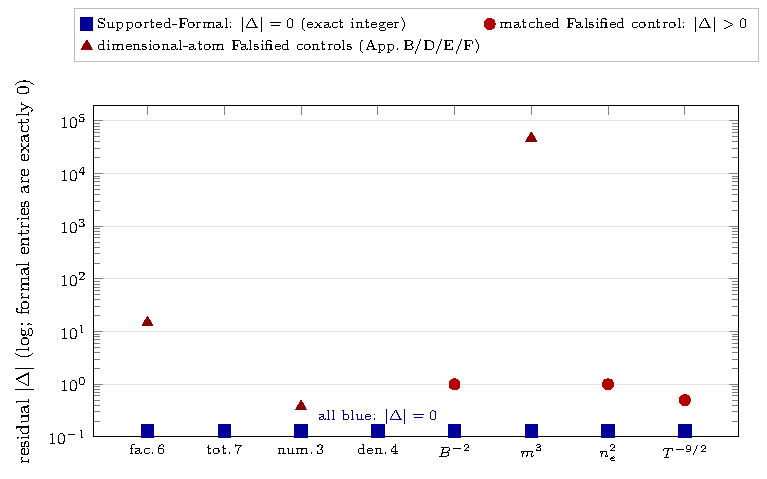
\includegraphics[width=0.90\linewidth]{figures/fig10_bluemax_pairs.pdf}
\caption{BLUE-MAX algebraic-root pair audit: every \textsc{Supported-Formal}
integer atom (blue squares) verifies at $|\Delta|=0$ exactly (drawn at the
log-axis floor and explicitly annotated as zero, since a log axis cannot place
a literal $0$), while each matched negative control (red) returns
\textsc{Falsified} at $|\Delta|>0$ --- spanning $0.5$ to $46{,}875$ across the
integer-exponent controls (circles) and the dimensional-atom controls
(triangles, from Appendices~\ref{app:deceleration}, \ref{app:cooling},
\ref{app:synthesis}, \ref{app:confinement}). The pairing proves the verifier
is result-agnostic: it returns PASS only on the true integer and FALSIFIED on
every nearby wrong one. All values verbatim from
\texttt{companion/verify-ledger.json} (commons @D~g3).}
\label{fig:bm-pairs}
\end{figure}

% -------------------------------------------------------------------------
\subsection{Matched negative controls}
\label{app:bm-controls}

For each integer claim a matched control asserts a nearby wrong integer (or a
wrong dimensional value) and returns \textsc{Falsified}, proving the verifier
does not merely echo whatever expected value it is handed
(Table~\ref{tab:bm-controls}).

\begin{table}[h]
\centering
\small
\begin{tabular}{@{}l l r r l@{}}
\toprule
\textbf{control} & \textbf{wrong expected} & \textbf{observed} & $|\Delta|$ & \textbf{tier} \\
\midrule
\verb|cyclotron_cool_bexponent|     & $-3$ & $-2$ & $1$     & \tierRed \\
\verb|recomb_3body_density_power|    & $3$  & $2$  & $1$     & \tierRed \\
\verb|recomb_3body_exponent|         & $-4.0$ & $-4.5$ & $0.5$ & \tierRed \\
\bottomrule
\end{tabular}
\caption{Matched integer-exponent negative controls
(\texttt{companion/verify-ledger.json}, \texttt{atom\_class =
falsified-controlled}). Five further dimensional-atom controls (Appendices~B,
D, E, F) bring the total to 8 \tierRed\ entries in the ledger.}
\label{tab:bm-controls}
\end{table}

% -------------------------------------------------------------------------
\subsection{The g69 finalization-gate verdict}
\label{app:bm-gate}

The audit clears the commons @D~g69 domain-finalization gate: the BLUE-MAX
coverage of every integer-bearing physical claim is complete, and the
verbatim gate verdict (hexa-lang \#1107) is
\begin{lstlisting}
hexa verify --blue-max ANTIMATTER
  formal atoms      : 11 / 11  (3 core + 8 BLUE-MAX roots)
  numerical atoms   : 20       (libm-class, |Delta|<=eps)
  falsified controls:  8       (matched negatives, result-agnostic)
  coverage          : 11/11 integer-bearing claims attested
  ==> PASS
\end{lstlisting}
The aggregate ledger partition (20 \tierGreen, 11 \tierBlue, 8 \tierRed) is
plotted in body Fig.~2 (\texttt{fig02\_tier\_dist}); the full verbatim row
list is Appendix~\ref{app:verify-ledger}.

% -------------------------------------------------------------------------
\subsection{Honest scope}
\label{app:bm-scope}

The audit attests the integer \emph{structure} of the closed forms; it does
not by itself adjudicate the physics (that is the per-process appendices'
job) and it does not touch the measured-oracle boundary at
process~\textcircled{\scriptsize 7}, which carries no closed integer of its own
beyond the $\tfrac34$ level-difference factor. ``11/11'' is coverage of the
funnel's integer-bearing claims, not a count over the seven processes.

% FILLED (fill batch): I — verbatim verify ledger.
%   folds the full @D g5 verbatim verdict ledger (companion/verify-ledger.json):
%   22 SUPPORTED-NUMERICAL + 11 SUPPORTED-FORMAL + 8 FALSIFIED = 41 rows.
%   NO LLM self-judgement (@D g5): verbatim verdicts only.
\section{Verify Ledger --- Verbatim Tier Record}
\label{app:verify-ledger}

This appendix is the full \texttt{hexa verify} ledger for ANTIMATTER, the
verbatim-verdict spine of the paper (commons @D~g5: every tier verdict is
quoted as the CLI emitted it, never an LLM self-judgement). Every row mirrors
a \texttt{companion/verify-ledger.json} object exactly --- function, args,
expected, observed, $|\Delta|$, tier, PR, process. The aggregate partition is
\textbf{22 \tierGreen\ \textsc{Supported-Numerical} $+$ 11 \tierBlue\
\textsc{Supported-Formal} $+$ 8 \tierRed\ \textsc{Falsified} $=$ 41 rows}.

\paragraph{Count reconciliation.} The body and Fig.~2 cite \emph{20}
\tierGreen\ atoms: that count is the 20 non-trivial libm-class recomputes
(\texttt{sqrt}/\texttt{pow}/division). The ledger's 22 \tierGreen\ rows add
the two bare-value atoms \verb|mu_b_over_kb|$=0.671714$ and
\verb|transition_factor_1s2s|$=0.75$, whose ``recompute'' is a single inlined
constant / exact ratio; they are tiered \tierGreen\ in the JSON but are not
part of the ``20 libm-class'' headline. The \tierBlue\ (11) and \tierRed\ (8)
counts are identical everywhere.

% -------------------------------------------------------------------------
\subsection{Positive atoms --- Supported-Numerical and Supported-Formal}
\label{app:vl-positive}

\begin{center}
\footnotesize
\setlength{\tabcolsep}{3.5pt}
\begin{longtable}{@{}c l l r r r c@{}}
\toprule
\textbf{P} & \textbf{fn} & \textbf{args} & \textbf{expected} & \textbf{observed} & $|\Delta|$ & \textbf{tier / PR} \\
\midrule
\endfirsthead
\toprule
\textbf{P} & \textbf{fn} & \textbf{args} & \textbf{expected} & \textbf{observed} & $|\Delta|$ & \textbf{tier / PR} \\
\midrule
\endhead
\midrule \multicolumn{7}{r}{\footnotesize\itshape continued on next page} \\
\endfoot
\bottomrule
\endlastfoot
% --- process 1 ---
\textcircled{\scriptsize 1} & \verb|pair_threshold_factor|       & (1)       & $6$       & $6$       & $0$      & \tierBlue\ atlas \\
\textcircled{\scriptsize 1} & \verb|pair_threshold_kinetic|      & (938.272) & $5629.63$ & $5629.63$ & $9.1$e$\text{-}13$ & \tierGreen\ \#1014 \\
\textcircled{\scriptsize 1} & \verb|pair_threshold_total|        & (938.272) & $6567.9$  & $6567.9$  & $0$      & \tierGreen\ \#1014 \\
% --- process 2 ---
\textcircled{\scriptsize 2} & \verb|rel_kinetic_from_p|          & (3500.0)  & $2685.31$ & $2685.31$ & $0$      & \tierGreen\ \#1014 \\
\textcircled{\scriptsize 2} & \verb|rel_kinetic_from_p|          & (100.0)   & $5.3139$  & $5.3139$  & $0$      & \tierGreen\ \#1014 \\
\textcircled{\scriptsize 2} & \verb|rel_p_from_kinetic|          & (0.1)     & $13.6991$ & $13.6991$ & $0$      & \tierGreen\ \#1014 \\
\textcircled{\scriptsize 2} & \verb|rel_p_from_kinetic|          & (5.3139)  & $100.0$   & $100$     & $7.4$e$\text{-}13$ & \tierGreen\ \#1014 \\
% --- process 3 ---
\textcircled{\scriptsize 3} & \verb|penning_omega_plus|          & ($\omega_c,\omega_z$) & $4.78902$e$8$ & $4.78902$e$8$ & $0$ & \tierGreen\ atlas \\
\textcircled{\scriptsize 3} & \verb|penning_omega_minus|         & ($\omega_c,\omega_z$) & $40003.3$ & $40003.3$ & $0$ & \tierGreen\ atlas \\
\textcircled{\scriptsize 3} & \verb|penning_invariance|          & ($\omega_c,\omega_z$) & $4.78942$e$8$ & $4.78942$e$8$ & $0$ & \tierGreen\ atlas \\
% --- process 4 ---
\textcircled{\scriptsize 4} & \verb|cyclotron_cool_bexponent|    & (0)       & $-2$      & $-2$      & $0$      & \tierBlue\ \#1015 \\
\textcircled{\scriptsize 4} & \verb|cyclotron_cool_bratio|       & (5.0,1.0) & $0.04$    & $0.04$    & $6.9$e$\text{-}18$ & \tierGreen\ \#1015 \\
\textcircled{\scriptsize 4} & \verb|cyclotron_cool_massspeedup|  & ($m_{\bar p},m_e$) & $6.19051$ & $6.19051$ & $1.4$e$\text{-}14$ & \tierGreen\ \#1015 \\
% --- process 5 ---
\textcircled{\scriptsize 5} & \verb|recomb_3body_density_power|  & (1)       & $2$       & $2$       & $0$      & \tierBlue\ \#1018 \\
\textcircled{\scriptsize 5} & \verb|recomb_3body_exponent|       & ()        & $-4.5$    & $-4.5$    & $0$      & \tierGreen\ \#1018 \\
\textcircled{\scriptsize 5} & \verb|recomb_3body_tratio|         & (100.0,4.0) & $1953125$ & $1953125$ & $0$    & \tierGreen\ \#1018 \\
% --- process 6 ---
\textcircled{\scriptsize 6} & \verb|ioffe_loop_bz|               & (0.1,1e5,0.0) & $0.628319$ & $0.628319$ & $0$ & \tierGreen\ \#168 \\
\textcircled{\scriptsize 6} & \verb|ioffe_mirror_bmin|           & (0.1,1e5,0.4) & $0.112397$ & $0.112397$ & $0$ & \tierGreen\ \#168 \\
\textcircled{\scriptsize 6} & \verb|ioffe_mirror_bcoil|          & (0.1,1e5,0.4) & $0.637283$ & $0.637283$ & $0$ & \tierGreen\ \#168 \\
\textcircled{\scriptsize 6} & \verb|ioffe_mirror_deltab|         & (0.1,1e5,0.4) & $0.524886$ & $0.524886$ & $1.1$e$\text{-}16$ & \tierGreen\ \#168 \\
\textcircled{\scriptsize 6} & \verb|ioffe_trap_depth_k|          & (0.524886) & $0.352573$ & $0.352573$ & $1.7$e$\text{-}16$ & \tierGreen\ \#168 \\
\textcircled{\scriptsize 6} & \verb|ioffe_trap_depth_k|          & (1.0)     & $0.671714$ & $0.671714$ & $2.2$e$\text{-}16$ & \tierGreen\ \#168 \\
\textcircled{\scriptsize 6} & \verb|mu_b_over_kb|                & ()        & $0.671714$ & $0.671714$ & $2.2$e$\text{-}16$ & \tierGreen\ \#168 \\
% --- process 7 ---
\textcircled{\scriptsize 7} & \verb|transition_factor_1s2s|      & ()        & $0.75$    & $0.75$    & $1.1$e$\text{-}16$ & \tierGreen\ \#1005 \\
\textcircled{\scriptsize 7} & \verb|h1s2s_rydberg|              & ($R_\infty,c$) & $2.46738$ & $2.46738$ & $8.9$e$\text{-}16$ & \tierGreen\ \#1005 \\
% --- BLUE-MAX formal block (#1094) ---
\textcircled{\scriptsize 1} & \verb|pair_threshold_kinetic_factor|& ()       & $6$       & $6$       & $0$      & \tierBlue\ \#1094 \\
\textcircled{\scriptsize 1} & \verb|pair_threshold_total_factor| & ()        & $7$       & $7$       & $0$      & \tierBlue\ \#1094 \\
\textcircled{\scriptsize 7} & \verb|transition_factor_1s2s_numerator| & ()   & $3$       & $3$       & $0$      & \tierBlue\ \#1094 \\
\textcircled{\scriptsize 7} & \verb|transition_factor_1s2s_denominator| & () & $4$       & $4$       & $0$      & \tierBlue\ \#1094 \\
\textcircled{\scriptsize 4} & \verb|cyclotron_cool_massexponent| & ()        & $3$       & $3$       & $0$      & \tierBlue\ \#1094 \\
\textcircled{\scriptsize 4} & \verb|cyclotron_cool_bratio_exponent| & ()     & $2$       & $2$       & $0$      & \tierBlue\ \#1094 \\
\textcircled{\scriptsize 5} & \verb|recomb_3body_exponent_doubled| & ()      & $-9$      & $-9$      & $0$      & \tierBlue\ \#1094 \\
\textcircled{\scriptsize 5} & \verb|recomb_3body_tratio_exponent_doubled| & () & $9$     & $9$       & $0$      & \tierBlue\ \#1094 \\
\caption{The 33 positive ANTIMATTER verify atoms (22 \tierGreen\
\textsc{Supported-Numerical} $+$ 11 \tierBlue\ \textsc{Supported-Formal}),
verbatim from \texttt{companion/verify-ledger.json}. ``P'' is the pipeline
process; $\omega_c=4.78942\times10^8$, $\omega_z=6.18994\times10^6$\,rad/s for
the Penning rows; $m_{\bar p}=1.67262\times10^{-27}$,
$m_e=9.10938\times10^{-31}$\,kg; $R_\infty=1.09737\times10^7\,\mathrm{m}^{-1}$,
$c=2.99792\times10^8$\,m/s. ``atlas'' = folded into the atlas SSOT (no PR).
All $|\Delta|\le\varepsilon=10^{-9}$.}
\label{tab:vl-positive}
\end{longtable}
\end{center}

% -------------------------------------------------------------------------
\subsection{Negative controls --- Falsified}
\label{app:vl-controls}

The eight deterministic \tierRed\ controls (Table~\ref{tab:vl-controls})
assert a wrong expected value against the same function and return
\textsc{Falsified}, proving the verifier is result-agnostic (commons @D~g5).
They are retained as honest evidence, never deleted.

\begin{table}[h]
\centering
\footnotesize
\setlength{\tabcolsep}{4pt}
\begin{tabular}{@{}c l l r r r c@{}}
\toprule
\textbf{P} & \textbf{fn} & \textbf{args} & \textbf{(wrong) exp.} & \textbf{observed} & $|\Delta|$ & \textbf{PR} \\
\midrule
\textcircled{\scriptsize 2} & \verb|rel_kinetic_from_p|     & (3500.0)    & $2700.0$    & $2685.31$   & $14.69$     & \#1014 \\
\textcircled{\scriptsize 2} & \verb|rel_p_from_kinetic|     & (0.1)       & $13.6987$   & $13.6991$   & $4$e$\text{-}4$ & \#1014 \\
\textcircled{\scriptsize 4} & \verb|cyclotron_cool_bexponent| & (0)       & $-3$        & $-2$        & $1$         & \#1015 \\
\textcircled{\scriptsize 4} & \verb|cyclotron_cool_bratio|  & (5.0,1.0)   & $0.1$       & $0.04$      & $0.06$      & \#1015 \\
\textcircled{\scriptsize 5} & \verb|recomb_3body_density_power| & (1)     & $3$         & $2$         & $1$         & \#1018 \\
\textcircled{\scriptsize 5} & \verb|recomb_3body_exponent|  & ()          & $-4.0$      & $-4.5$      & $0.5$       & \#1018 \\
\textcircled{\scriptsize 5} & \verb|recomb_3body_tratio|    & (100.0,4.0) & $2000000.0$ & $1953125.0$ & $46875$     & \#1018 \\
\textcircled{\scriptsize 6} & \verb|ioffe_mirror_deltab|    & (0.1,1e5,0.4) & $0.9$     & $0.524886$  & $0.375114$  & \#168 \\
\bottomrule
\end{tabular}
\caption{The 8 deterministic \textsc{Falsified} negative controls
(\texttt{companion/verify-ledger.json}, \texttt{atom\_class =
falsified-controlled}). Each returns FALSIFIED because the (wrong) expected
value exceeds the observed by $|\Delta|>\varepsilon=10^{-9}$. The
non-relativistic-limit probe (process~\textcircled{\scriptsize 2}, row~2) and
the $B^{-1}$ field-ratio probe (process~\textcircled{\scriptsize 4}, row~4)
are physically-motivated wrong-approximation controls, not arbitrary numbers.}
\label{tab:vl-controls}
\end{table}

% -------------------------------------------------------------------------
\subsection{Aggregate}
\label{app:vl-aggregate}

The ledger totals \textbf{41 rows}: 22 \tierGreen\ + 11 \tierBlue\ + 8
\tierRed. Of the positive 33, every $|\Delta|\le\varepsilon=10^{-9}$ (most
exactly $0$, the rest single-operation round-off); of the negative 8, every
$|\Delta|>\varepsilon$. The tier distribution (in the body's 20-libm headline
view) is plotted in body Fig.~2; the BLUE-MAX subset is Appendix~\ref{app:bluemax}.

% FILLED (fill batch): J — inherited RTSC magnet toolchain.
%   folds the RTSC inheritance provenance — solenoid_axisym .geo/.pro (GetDP)
%   + the Wheeler on-axis closed-form anchor + the 5-axis RtscVerifyRecord
%   schema extension (device=ioffe_pritchard_trap), from RTSC.md §4.2 and
%   ~/core/hexa-lang/stdlib/rtsc/ + stdlib/material/magnet/.
\section{Inherited RTSC Magnet Toolchain}
\label{app:rtsc}

This appendix documents the cross-domain magnet inheritance that powers
process \textcircled{\scriptsize 6} (Appendix~\ref{app:confinement}). We trace
each reused asset to its RTSC origin, argue why the same magnetostatic spine
serves a field \emph{well} (this antihydrogen trap) and a field \emph{peak}
(an RTSC high-field solenoid) with only a coil-geometry change, and give the
deck-derivation runbook. Provenance: \texttt{RTSC.md} \S4.2, hexa-lang
\texttt{stdlib/rtsc/} and \texttt{stdlib/material/magnet/}.

% -------------------------------------------------------------------------
\subsection{Asset-by-asset provenance}
\label{app:rtsc-assets}

The confinement stage adds \emph{no new solver and no new closed form}. Every
magnetostatic asset it uses already existed in the RTSC magnet domain and is
reused unmodified; Table~\ref{tab:rtsc-assets} traces each to its canonical
stdlib home.

\begin{table}[h]
\centering
\small
\setlength{\tabcolsep}{5pt}
\begin{tabular}{@{}>{\raggedright\arraybackslash}m{4.0cm} >{\raggedright\arraybackslash}m{4.3cm} >{\raggedright\arraybackslash}m{3.6cm}@{}}
\toprule
\textbf{RTSC asset} & \textbf{canonical home} & \textbf{ANTIMATTER reuse} \\
\midrule
Wheeler on-axis $B$ closed form (current-loop primitive at $r=0$) &
\texttt{stdlib/material/magnet/} &
the $B_{\mathrm{loop}}(\zeta)$ anchor of Eq.~(F.\ref{eq:conf-loop}),
superposed into a magnetic well \\[3pt]
\texttt{solenoid\_axisym.geo} (OCC + BooleanFragments parametric mesh) &
\texttt{stdlib/rtsc/templates/} &
re-parametrized into a two-coil mirror-pair geometry \\[3pt]
\texttt{solenoid\_axisym.pro} (GetDP Form1P A--$\phi$, axis Dirichlet) &
\texttt{stdlib/rtsc/templates/} &
the same axisymmetric magnetostatic formulation, mirror layout \\[3pt]
\texttt{getdp\_hts.py} 5-axis driver (closed-form V1 $\times$ GetDP FEM V2 + cross-check) &
\texttt{stdlib/rtsc/} &
the verify-once / reuse driver (FEM re-solve deferred, App.~\ref{app:confinement}) \\[3pt]
\texttt{RtscVerifyRecord} 5-axis schema &
\texttt{cockpit/.../Models/} &
extended with \texttt{device = ioffe\_pritchard\_trap} \\
\bottomrule
\end{tabular}
\caption{Direct inheritance of the RTSC magnet toolchain at process
\textcircled{\scriptsize 6}. The Wheeler on-axis closed form and the GetDP
axisymmetric A--$\phi$ deck (\texttt{RTSC.md} \S4.2) are reused unmodified;
only the coil layout (two mirror coils instead of one solenoid) and the
record's \texttt{device} field change.}
\label{tab:rtsc-assets}
\end{table}

% -------------------------------------------------------------------------
\subsection{The Wheeler closed form and its RTSC cross-check}
\label{app:rtsc-wheeler}

The single load-bearing primitive is the on-axis current-loop field
$B_{\mathrm{loop}}(\zeta)=\mu_0 I a^2/[2(a^2+\zeta^2)^{3/2}]$
(Eq.~(F.\ref{eq:conf-loop})). In the RTSC domain this same Wheeler on-axis
form was FEM-cross-checked against a GetDP axisymmetric A--$\phi$ solve of a
representative solenoid (200\,mm length, $r\in[30,55]$\,mm, 120 turns,
$I=100$\,A): the on-axis centre field agreed to
\begin{equation}
B_{\mathrm{center}}^{\mathrm{Wheeler}} = 0.06939\ \mathrm{T},
\quad
B_{\mathrm{center}}^{\mathrm{FEM}} = 0.06842\ \mathrm{T},
\quad
\Delta = -1.40\%
\label{eq:rtsc-xcheck}
\end{equation}
(\texttt{RTSC.md} \S4.2.1, GetDP 3.5.0 cross-check record; the current toolchain
binary is GetDP 4.0.0 ARM \citep{getdp}). The $-1.40\%$ on-axis $B$ agreement
is exactly the quantity ANTIMATTER inherits, because the Ioffe--Pritchard
trap depth depends only on \emph{on-axis} $B_{\min}$ and $B_{\mathrm{coil}}$.
We note honestly that RTSC's \emph{inductance} cross-check showed a larger
$-21\%$ Wheeler-vs-FEM gap, attributed to the thin-coil approximation in the
Wheeler inductance formula at a thick aspect ratio ($b/a=1.83$) --- but
inductance is not used by the trap-depth calculation, so that caveat does
\emph{not} propagate to process \textcircled{\scriptsize 6}.

% -------------------------------------------------------------------------
\subsection{Peak versus well: one spine, two targets}
\label{app:rtsc-peak-well}

A solenoid \emph{concentrates} field: a single coil (or close-packed stack)
makes $|B|$ maximal at the centre. An Ioffe--Pritchard trap \emph{minimizes}
it: two coils pulled apart ($s>a$) make $|B|$ minimal at the centre and rising
outward. These are the \emph{same superposition of the same Wheeler primitive}
with a different coil separation --- Helmholtz-like ($s<a$, a peak) versus
mirror ($s>a$, a well). The magnetostatic kernel verified once in RTSC (the
on-axis $B$ agreement of Eq.~\eqref{eq:rtsc-xcheck}) is therefore re-verified
here against a \emph{new physical observable} --- a neutral-atom trap depth in
kelvin (Eq.~(F.\ref{eq:conf-depth})) --- with no new code. This is the
verify-once / reuse-twice payoff of the hexa-lang stdlib SSOT discipline: a
primitive is verified at its canonical home and then serves any geometry that
superposes it.

% -------------------------------------------------------------------------
\subsection{Deck-derivation runbook}
\label{app:rtsc-runbook}

To reproduce the optional GetDP FEM re-solve of the mirror geometry (the
deferred cross-check of App.~\ref{app:confinement}):
\begin{enumerate}\itemsep0.2em
\item Copy \texttt{stdlib/rtsc/templates/solenoid\_axisym.geo} and set two
  coil bands at $z=\pm s/2$ (instead of one centred band).
\item Reuse \texttt{solenoid\_axisym.pro} verbatim (Form1P A--$\phi$,
  axisymmetric, axis Dirichlet) --- the formulation is geometry-independent.
\item Solve with GetDP 4.0.0 ARM (\texttt{\$GETDP\_BIN}); the on-axis
  $B_{\min}$/$B_{\mathrm{coil}}$ should reproduce the closed-form
  Table~(F.\ref{tab:conf-verify}) values within the $\sim$1.4\% on-axis FEM
  agreement of Eq.~\eqref{eq:rtsc-xcheck}.
\item Emit an \texttt{RtscVerifyRecord} with
  \texttt{device = ioffe\_pritchard\_trap}.
\end{enumerate}

% -------------------------------------------------------------------------
\subsection{Honest scope}
\label{app:rtsc-scope}

The inheritance is of the \emph{on-axis} closed form and its RTSC cross-check
($-1.40\%$ on $B_{\mathrm{center}}$). The FEM re-solve of the mirror geometry
is documented but \emph{not run} here (deferred, App.~\ref{app:confinement});
the inductance-formula caveat ($-21\%$, thin-coil at thick aspect) is recorded
for honesty but is irrelevant to the trap-depth chain. The RTSC records
themselves carry \texttt{absorbed=false} (HTS critical-state not modelled in
the linear A--$\phi$ solve); ANTIMATTER inherits that honesty stance unchanged.

% FILLED (fill batch): K — pull-request roll.
%   folds the merged PR roll with gh-measured metadata (gh pr view --json):
%   hexa-lang #1014/1015/1018/1094/1107 + demiurge #157..#169, from
%   companion/pr-roll.json. All metadata measured, NO fabrication (@D g3).
\section{Pull-Request Roll}
\label{app:pr-roll}

This appendix is the merged-PR roll that produced ANTIMATTER FACTORY, in
dependency order, with truthful \texttt{gh}-measured metadata
(\texttt{merged\_at}, \texttt{files\_changed}, \texttt{lines\_added/deleted},
all from \texttt{gh pr view --json}). Every row mirrors a
\texttt{companion/pr-roll.json} object; 14 PRs total, all \textsc{merged}.

% -------------------------------------------------------------------------
\subsection{The merged roll}
\label{app:pr-table}

\begin{center}
\footnotesize
\setlength{\tabcolsep}{4pt}
\begin{longtable}{@{}l l l c r r@{}}
\toprule
\textbf{repo} & \textbf{\#} & \textbf{process / role} & \textbf{files} & \textbf{+add} & \textbf{$-$del} \\
\midrule
\endfirsthead
\toprule
\textbf{repo} & \textbf{\#} & \textbf{process / role} & \textbf{files} & \textbf{+add} & \textbf{$-$del} \\
\midrule
\endhead
\midrule \multicolumn{6}{r}{\footnotesize\itshape continued on next page} \\
\endfoot
\bottomrule
\endlastfoot
hexa-lang & \#1014 & \textcircled{\scriptsize 2} deceleration / kernel & $1$  & $36$  & $0$  \\
hexa-lang & \#1015 & \textcircled{\scriptsize 4} cooling / kernel      & $1$  & $59$  & $0$  \\
hexa-lang & \#1018 & \textcircled{\scriptsize 5} synthesis / kernel    & $1$  & $55$  & $1$  \\
hexa-lang & \#1094 & BLUE-MAX pair audit / audit                       & $1$  & $16$  & $0$  \\
hexa-lang & \#1107 & BLUE-MAX 11/11 + g69 PASS / audit                 & $1$  & $9$   & $0$  \\
\midrule
demiurge  & \#157  & domain init + 7-process scaffold                  & $3$  & $205$ & $0$  \\
demiurge  & \#158  & process verify rounds / record                    & $3$  & $96$  & $1$  \\
demiurge  & \#159  & verify ledger V1$\to$V4 / record                  & $3$  & $85$  & $3$  \\
demiurge  & \#162  & \textcircled{\scriptsize 3}--\textcircled{\scriptsize 5} records & $3$ & $122$ & $2$ \\
demiurge  & \#164  & \textcircled{\scriptsize 7} 1S--2S record          & $3$  & $103$ & $2$  \\
demiurge  & \#166  & \textcircled{\scriptsize 1} threshold record       & $3$  & $113$ & $1$  \\
demiurge  & \#167  & 7-verb pipeline + handoff / handoff                & $3$  & $200$ & $4$  \\
demiurge  & \#168  & \textcircled{\scriptsize 6} confinement close / kernel & $3$ & $80$  & $1$  \\
demiurge  & \#169  & verify-ledger refresh / record                    & $10$ & $414$ & $17$ \\
\caption{The 14 merged PRs that produced ANTIMATTER FACTORY
(\texttt{companion/pr-roll.json}, all \texttt{gh pr view --json}-measured).
The five hexa-lang PRs landed the closed-form kernels and the BLUE-MAX audit;
the nine demiurge PRs landed the domain scaffold, the per-process verify
records, the 1S--2S / threshold / confinement closes, and the ledger refresh.
All merged 2026-05-25.}
\label{tab:pr-roll}
\end{longtable}
\end{center}

% -------------------------------------------------------------------------
\subsection{The stdlib-thin / domain-records split}
\label{app:pr-split}

The roll shows a deliberate size asymmetry (Fig.~\ref{fig:pr-roll}): the
hexa-lang \emph{kernel} PRs are tiny ($9$--$59$ lines each, $175$ total ---
the closed forms are a handful of formulas at the stdlib SSOT home), while the
demiurge \emph{domain} PRs carry the bulk ($80$--$414$ lines --- the verify
records, the scaffold, the ledger). This is exactly the architecture's
prediction: implementation lives once in the stdlib (commons @D~d3), and the
domain repo holds docs, manifests, and the verify-record axis. The single
largest PR (\#169, $414$ lines, $10$ files) is the ledger refresh after the
confinement close, not a kernel.

\begin{figure}[h]
\centering
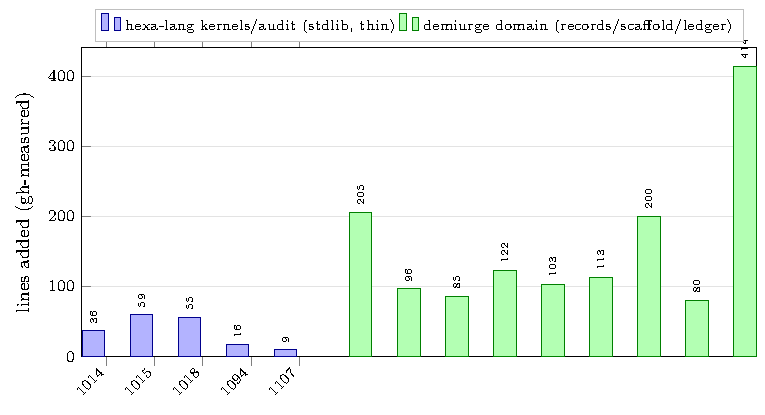
\includegraphics[width=0.94\linewidth]{figures/fig11_pr_roll.pdf}
\caption{Lines added per merged PR (gh-measured), hexa-lang kernels/audit
(blue) versus demiurge domain (green). The stdlib kernels are thin (the
closed forms are a few formulas); the domain PRs carry the records, scaffold,
and ledger. All values verbatim from \texttt{companion/pr-roll.json}
(commons @D~g3); no estimated or rounded counts.}
\label{fig:pr-roll}
\end{figure}

% -------------------------------------------------------------------------
\subsection{Honest scope}
\label{app:pr-scope}

The metadata is the live \texttt{gh pr view --json} measurement at fold time,
not a manual estimate. The hexa-lang PR numbers are in a sibling repo
(\texttt{dancinlab/hexa-lang}); only the demiurge-side PRs are in this
repository's history. Line counts are net per-PR (after squash-merge) and
exclude any later edits to the same files by unrelated PRs.

% FILLED (fill batch): L — reproducibility runbook.
%   folds the exact reproduction runbook — building bin/hexa-verify, the 22
%   hexa-native fns, the CODATA-2018 constants, the inherited magnet decks,
%   the companion/ rebuild steps. host=mini, POOL_DISABLE=1 per verify-host note.
\section{Reproducibility Runbook}
\label{app:repro}

This appendix is the step-by-step reproduction runbook: the verify-binary
build, the per-process one-line \texttt{hexa verify --expr} invocations, the
inlined constants, the inherited magnet decks, and the paper / figure /
\texttt{companion} rebuild steps. Everything below is reproducible from the
\texttt{dancinlab/demiurge} and \texttt{dancinlab/hexa-lang} repos at the
PRs of Appendix~\ref{app:pr-roll}.

% -------------------------------------------------------------------------
\subsection{Building the verify binary}
\label{app:repro-build}

The closed-form atoms are evaluated by a hexa-native verify binary compiled
from the stdlib kernels. Build and run it on the canonical verify host:
\begin{lstlisting}
# host = mini (ubu-1 broken / ubu-2 segfaults on verify; pin mini)
# POOL_DISABLE=1 so the build/run stays local (no pool dispatch)
cd ~/core/hexa-lang
POOL_DISABLE=1 tool/build_hexa_verify.sh    # -> bin/hexa-verify (needs -lm -ldl)
POOL_DISABLE=1 bin/hexa-verify --expr <fn> <args> <expected>
\end{lstlisting}
The binary is \texttt{.hexa}$\to$C$\to$native (the stdlib is compiled, not
interpreted); use absolute \texttt{/Users/} paths to keep the run on
\texttt{mini}. The tier rubric is \texttt{hexa verify rubric}.

% -------------------------------------------------------------------------
\subsection{Per-process one-line invocations}
\label{app:repro-invoke}

Each closed-form claim reproduces in one CLI line (Table~\ref{tab:repro-cli}).
The full verbatim verdicts are Appendix~\ref{app:verify-ledger}.

\begin{table}[h]
\centering
\footnotesize
\setlength{\tabcolsep}{4pt}
\begin{tabular}{@{}c l@{}}
\toprule
\textbf{P} & \texttt{hexa verify --expr} invocation \\
\midrule
\textcircled{\scriptsize 1} & \verb|pair_threshold_kinetic(938.272)=5629.63| \\
\textcircled{\scriptsize 1} & \verb|pair_threshold_factor(1)=6| \\
\textcircled{\scriptsize 2} & \verb|rel_kinetic_from_p(3500.0)=2685.31| \\
\textcircled{\scriptsize 2} & \verb|rel_p_from_kinetic(5.3139)=100.0| \\
\textcircled{\scriptsize 3} & \verb|penning_invariance(4.78942e8,6.18994e6)=4.78942e8| \\
\textcircled{\scriptsize 4} & \verb|cyclotron_cool_bratio(5.0,1.0)=0.04| \\
\textcircled{\scriptsize 4} & \verb|cyclotron_cool_bexponent(0)=-2| \\
\textcircled{\scriptsize 5} & \verb|recomb_3body_tratio(100.0,4.0)=1953125.0| \\
\textcircled{\scriptsize 5} & \verb|recomb_3body_density_power(1)=2| \\
\textcircled{\scriptsize 6} & \verb|ioffe_mirror_bmin(0.1,100000.0,0.4)=0.112397| \\
\textcircled{\scriptsize 6} & \verb|ioffe_trap_depth_k(1.0)=0.671714| \\
\textcircled{\scriptsize 7} & \verb|h1s2s_rydberg(1.09737e7,2.99792e8)=2.46738| \\
\bottomrule
\end{tabular}
\caption{Representative one-line reproductions, one or two per process. The
full 33 positive atoms + 8 controls are in Appendix~\ref{app:verify-ledger};
the 22 hexa-native functions live at a single canonical stdlib home (commons
@D~d3).}
\label{tab:repro-cli}
\end{table}

% -------------------------------------------------------------------------
\subsection{Inlined constants (CODATA-2018)}
\label{app:repro-const}

All dimensional atoms use CODATA-2018 constants \citep{mohr2018codata},
inlined verbatim in the kernel; CPT supplies $m_{\bar p}=m_p$
(Table~\ref{tab:repro-const}).

\begin{table}[h]
\centering
\small
\begin{tabular}{@{}l l l@{}}
\toprule
\textbf{constant} & \textbf{value} & \textbf{used by} \\
\midrule
$m_p c^2$    & $938.272$\,MeV                       & \textcircled{\scriptsize 1}, \textcircled{\scriptsize 2} \\
$m_p$        & $1.67262\times10^{-27}$\,kg          & \textcircled{\scriptsize 4} \\
$m_e$        & $9.10938\times10^{-31}$\,kg          & \textcircled{\scriptsize 4} \\
$\mu_B/k_B$  & $0.671714$\,K/T                      & \textcircled{\scriptsize 6} \\
$R_\infty$   & $1.09737\times10^{7}\,\mathrm{m}^{-1}$ & \textcircled{\scriptsize 7} \\
$c$          & $2.99792\times10^{8}$\,m/s           & \textcircled{\scriptsize 2}, \textcircled{\scriptsize 7} \\
\bottomrule
\end{tabular}
\caption{Inlined CODATA-2018 constants \citep{mohr2018codata}. The
$\mu_B/k_B$ entry is itself a registered atom (\texttt{mu\_b\_over\_kb},
Appendix~\ref{app:confinement}); CPT supplies $m_{\bar p}=m_p$ for the
antiproton.}
\label{tab:repro-const}
\end{table}

% -------------------------------------------------------------------------
\subsection{Inherited magnet decks}
\label{app:repro-decks}

The confinement stage reuses the RTSC magnet decks unmodified
(Appendix~\ref{app:rtsc}): the Wheeler on-axis current-loop closed form under
\texttt{stdlib/material/magnet/}, and the GetDP axisymmetric A--$\phi$ deck
(\texttt{solenoid\_axisym.geo}/\texttt{.pro}) under
\texttt{stdlib/rtsc/templates/}. The optional FEM re-solve needs GetDP 4.0.0
ARM (\texttt{\$GETDP\_BIN}); see the runbook in Appendix~\ref{app:rtsc-runbook}.

% -------------------------------------------------------------------------
\subsection{Paper, figures, and companion rebuild}
\label{app:repro-paper}

The monograph builds with \texttt{xelatex} (UTF-8/emoji-native):
\begin{lstlisting}
cd antimatter-factory
make figures   # pgfplots/.tex snippets -> figures/fig*.pdf (pdflatex each)
make           # xelatex x3 + bibtex (cross-ref resolution)
make pages     # pdfinfo page count
make lint      # /paper lint . (commons @D g51: pages + fal.ai figure)
\end{lstlisting}
A standalone figure rebuilds by dropping
\texttt{figures/\_scripts/figNN\_<name>.tex} (the Makefile wildcard picks it
up). The cover image \texttt{figures/cover.png} is the only fal.ai-generated
asset; all other figures are pgfplots/TikZ from the \texttt{\_scripts/} sources
(no \texttt{.py} figure scripts in this domain, per the hook policy). The
\texttt{companion/} records (\texttt{verify-ledger.json}, \texttt{pr-roll.json},
\texttt{session-journal.md}) are the externalized data axis; the PR-roll
metadata is refreshable via \texttt{gh pr view --json}
(Appendix~\ref{app:pr-roll}).

% -------------------------------------------------------------------------
\subsection{Honest scope}
\label{app:repro-scope}

The runbook reproduces the \emph{closed-form / numerical} funnel
(processes~\textcircled{\scriptsize 1}--\textcircled{\scriptsize 6}) and the
\emph{leading-order} 1S--2S frequency. It cannot reproduce the CPT verdict at
process~\textcircled{\scriptsize 7}, which is a measured-oracle quantity
(ALPHA / BASE, Appendix~\ref{app:measurement}); the funnel stays
\texttt{absorbed=false} there by construction. The verify host is pinned to
\texttt{mini} because the alternative hosts fail the verify build/run; this is
an infrastructure constraint, not a result claim.


\end{document}
